\documentclass[a4paper,12pt]{article}
\usepackage[T1]{fontenc}
\usepackage{imakeidx}
\usepackage{graphicx}

%\makeindex[columns=3, title=Alphabetical Index, intoc]

\usepackage{listings}

\begin{document}

\textbf{Networking}


\tableofcontents
\clearpage

\section{What it is}

A network is two or more \emph{computers} (or other electronic devices) that are \textbf{connected} together, usually by cables(guided) or Wi-Fi(unguided).

\section {benefits of a network}
\begin{enumerate}
\item {sharing hardware, such as printers, computers, phones, tablets, scanners, etc...}\footnotemark{}
\item {sharing software, allowing:}
    \begin{itemize}
    \item{multiple users to run the same programs on different computers}
    \item{data to be shared, so that other people can access shared work}
    \item{you to access your data from any computer on the network}
    \end{itemize}
\end{enumerate}

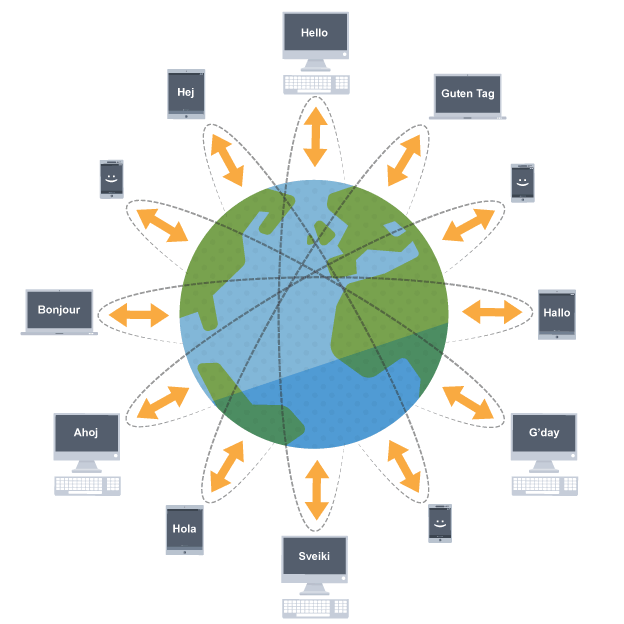
\includegraphics[width=11cm]{./net.png}
\footnotetext{All these pieces of hardware are usually addressed as \textbf{endpoints} as long as they have the ability to communicate effectively within a network}


Networking is crucial if you want to use your computer to communicate. Without it you couldn’t send an email, a text or an instant message and that would be so bad.

We use a huge network on a daily basis and this is called the internet. Around three billion people use the internet to share data, news and resources, amongst many other things.
\subsection{guided wiring}
Is quicker than unguided, it consists in physical wires. Optic Fiber is on the top of this list but can't be twisted. You can install a optic cable for a much longer distance and you won't get the same troubles you would get with copper cables for example

\subsection{unguided wiring}
This is Wi-Fi essentially. You can have a 2.4Ghz signal to reach longer distance but won't be nicely matched with a 5Ghz device

\section{LAN vs WAN}

LAN, which stands for local area network, and WAN, which stands for wide area network, are two types of networks that allow connection between computers. As the naming conventions suggest, LANs are for smaller, more localized networking — in a home, business, school, etc. — while WANs cover larger areas, such as cities, and even allow computers in different nations to connect. LANs are typically faster and more secure than WANs, but WANs enable more widespread connectivity

\clearpage

\section{IEEE 802.3}

IEEE 802.3 is a set of standards and protocols that define Ethernet-based networks. Ethernet technologies are primarily used in LANs, though they can also be used in WANs as well. IEEE 802.3 defines the physical layer and the medium access control (MAC) sub-layer of the data link layer for wired Ethernet networks.

\subesction{IEEE 802.3 Popular Versions}
There are a number of versions of IEEE 802.3 protocol. The most popular ones are.

\begin{itemize}
\item{IEEE 802.3: This was the original standard given for 10BASE-5. It used a thick single coaxial cable into which a connection can be tapped by drilling into the cable to the core. Here, 10 is the maximum throughput, i.e. 10 Mbps, BASE denoted use of baseband transmission, and 5 refers to the maximum segment length of 500m}
\item{IEEE 802.3a: This gave the standard for thin coax (10BASE-2), which is a thinner variety where the segments of coaxial cables are connected by BNC connectors. The 2 refers to the maximum segment length of about 200m (185m to be precise)}
\item{IEEE 802.3i: This gave the standard for twisted pair (10BASE-T) that uses unshielded twisted pair (UTP) copper wires as physical layer medium. The further variations were given by IEEE 802.3u for 100BASE-TX, 100BASE-T4 and 100BASE-FX}
\item{IEEE 802.3j: This gave the standard for Ethernet over Fiber (10BASE-F) that uses fiber optic cables as medium of transmission}
\end{itemize}
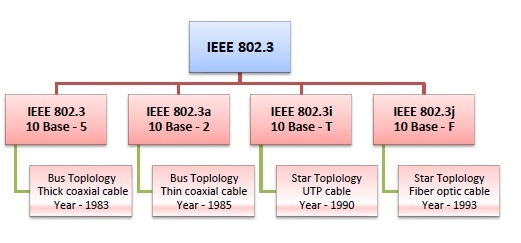
\includegraphics[width=15cm]{./ieee_802.jpg}

\section{Protocols}

Protocols are kind of rules defined in advance to make sure two or more devices know in advance what to expect if they send a particular message and what to expect in return 

\subsection{OSI standard}
The Open Systems Interconnection (OSI) model describes seven layers that computer systems use to communicate over a network. It was the first standard model for network communications, adopted by all major computer and telecommunication companies in the early 1980s

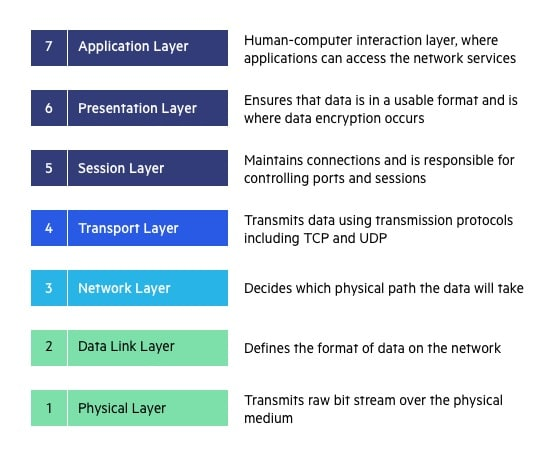
\includegraphics[width=13cm]{./OSI-7-layers.jpg}

The modern Internet is not based on OSI, but on the simpler TCP/IP model. However, the OSI 7-layer model is still widely used, as it helps visualize and communicate how networks operate, and helps isolate and troubleshoot networking problems.

OSI was introduced in 1983 by representatives of the major computer and telecom companies, and was adopted by ISO as an international standard in 1984.

\subsection{good mnemonic for OSI}
Every layer of the OSI model can be remembered with the mnemonic : Please Do Not Throw Sausage and Pizza Away

\subsection{theory vs practice}
Even if The Transmission Control Protocol/Internet Protocol (TCP/IP) model came before the Open Systems Interconnection (OSI) model it is what is used in practice today, and it has only five layers:

\begin{itemize}
\item {Application layer}
\item {Transport layer}
\item {Network access layer}
\item {Network interface layer}
\item {Hardware layer}
\end{itemize}

This may look drastically different from the OSI model, primarily because some functions are encompassed in a single layer: the application layer. In TCP/IP, this provides users with the physical standards, transport functions, network interface, and internetworking functions that correspond with the first three layers of the OSI model. In other words, in the TCP/IP model, these services are all done in the application layer.

TCP/IP is connection and connectionless

\subsection{horizontal vs vertical approach}
There's a debate on which one is vertical and which is horizontal so that point won't be discussed in this documents

\section{ARP/RARP/DHCP}
Address Resolution Protocol translates MAC addresses into IPs so that from the network layer we can communicate over the internet with IPs while RARP demands another computer (usually a server) to assign the demanding one with an IP which is essentially what DHCP is doing that's why RARP got obsolete
\subsection{ARP Tables}
These are used from every component in a network to know which MAC address the packet needs to point at 
On this machine for example all it needs to know is which is the MAC address of the gateway, and the TV who's connected in the same WiFi

\begin{lstlisting}
_gateway (192.168.0.1) at 24:a7:dc:31:5b:d1 [ether] on wlp3s0
TV (192.168.0.129) at cc:d3:c1:64:f9:f3 [ether] on wlp3s0
\end{lstlisting}

\subsection{Three-way-handshake}
This is when the client sends the ARP request to the server. The server does an aknowledgment and answers with an ARP reply saying both its MAC and its IP. It all happens like this :

When Computer 1 wants to talk to  Computer 2 in a local area network by Ethernet cables and network switches, with no intervening gateways or routers. Computer 1 has a packet to send to Computer 2. Through DNS, it determines that Computer 2 has the IP address 192.168.0.55.

To send the message, it also requires Computer 2's MAC address. First, Computer 1 uses a cached ARP table to look up 192.168.0.55 for any existing records of Computer 2's MAC address (00:EB:24:B2:05:AC). If the MAC address is found, it sends an Ethernet frame containing the IP packet onto the link with the destination address 00:EB:24:B2:05:AC. If the cache did not produce a result for 192.168.0.55, Computer 1 has to send a broadcast ARP request message (destination FF:FF:FF:FF:FF:FF MAC address), which is accepted by all computers on the local network, requesting an answer for 192.168.0.55.

Computer 2 responds with an ARP response message containing its MAC and IP addresses. As part of fielding the request, Computer 2 may insert an entry for Computer 1 into its ARP table for future use.

Computer 1 receives and caches the response information in its ARP table and can now send the packet

\clearpage

\section{Networking Hardware}
Computers need networking hardware in order to connect to each other. \textbf{Routers}, \textbf{hubs}, \textbf{switches} and \textbf{bridges} are all pieces of networking equipment that can perform slightly different tasks. A router can often incorporate hubs, switches and wireless access within the same hardware

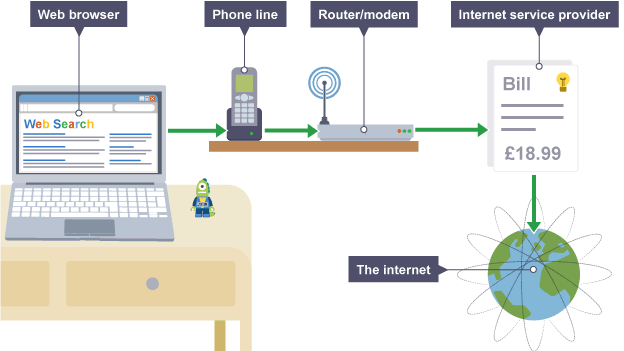
\includegraphics[width=13cm]{./large.PNG}

\subsection{Routers}
A router can form a \textbf{LAN} by connecting devices within a building. It also makes it possible to connect different networks together. Homes and businesses use a router to connect to the internet. A router can often incorporate a modem within the hardware.

\subsection{Modems}
A \textbf{modem} enables a computer to connect to the internet over a telephone line. A modem converts \textbf{digital} signals from a computer to analogue signals that are then sent down the telephone line. A modem on the other end converts the analogue signal back to a digital signal which another computer can understand.

\subsection{Hubs, bridges and switches}

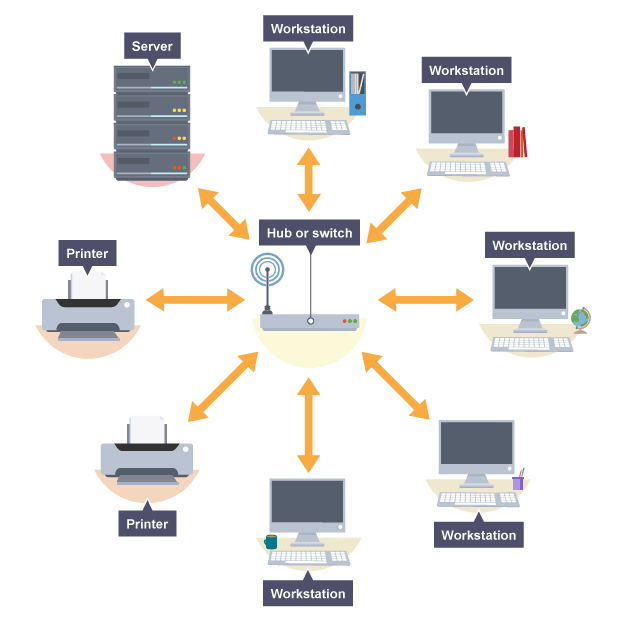
\includegraphics[width=13cm]{./hbs.PNG}

\textbf{Hubs}, \textbf{bridges} and \textbf{switches} allow multiple devices to connect to the router and they transfer data to all devices on a network. A router is a more complex device that usually includes the capability of hubs, bridges and switches.

\subsubsection{Hubs}
A hub broadcasts data to all devices on a network. This can use a lot of \textbf{bandwidth} as it results in unnecessary data being sent - not all computers might need to receive the data. A hub would be useful to link up a few games consoles for a local multiplayer game using a wired LAN.

\subsubsection{Bridges}
A \textbf{bridge} is used to connect two separate LAN networks. A computer can act as a bridge through the \textbf{operating system}. A bridge looks for the receiving device before it sends the message. This means that it will not send a message if the receiving computer is not there. It will check to see if the receiver has already had the message. This can help save unnecessary data transfers, which improves the performance of a network.

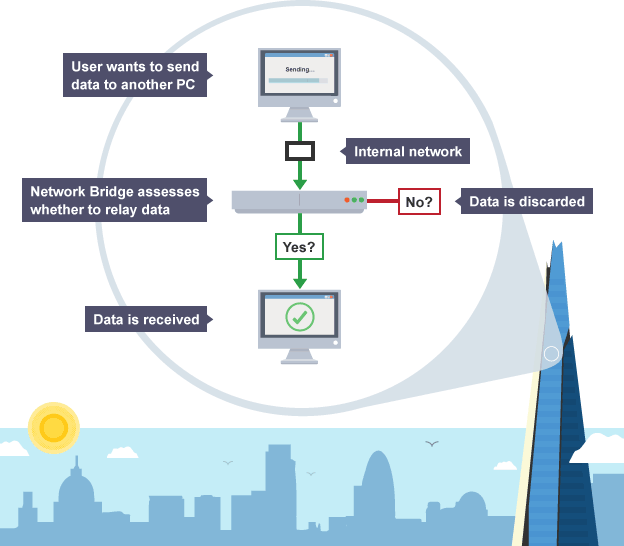
\includegraphics[width=13cm]{./performance.PNG}

\subsubsection{Switches}
A \textbf{switch} performs a similar role to a hub and a bridge but is more powerful. It stores the \textbf{MAC addresses} of devices on a network and filters \textbf{data packets} to see which devices have asked for them. This makes a switch more efficient when demand is high. If, for example, a game involved lots of data being passed between machines, then a switch could reduce the amount of \textbf{latency}

\section{Cisco Packet Tracer}

Packet Tracer is a cross-platform visual simulation tool designed by Cisco Systems that allows users to create network topologies and imitate modern computer networks. The software allows users to simulate the configuration of Cisco routers and switches using a simulated command line interface. Packet Tracer makes use of a drag and drop user interface, allowing users to add and remove simulated network devices as they see fit. The software is mainly focused towards Cisco Networking Academy students as an educational tool for helping them learn fundamental CCNA concepts. Previously students enrolled in a CCNA Academy program could freely download and use the tool free of charge for educational use.\footnotemark{} \newline

In this experiment we try to ping devices being set with 0 in the IP fields. Then we're gonna expand the network with more devices

\footnotetext{Bakni, Michel; Cardinale, Yudith; Moreno, Luis Manuel (June 2018). \textbf{An Approach to Evaluate Network Simulators: An Experience with Packet Tracer}.Revista Venezolana de Computación. 5: 29–36. ISSN 2244-7040. \newline Javid,Sheikh Raashid (May 2014). \textbf{Role of Packet Tracer in learning Computer Networks} (PDF). International Journal of Advanced Research in Computer and Communication Engineering. 3 (5): 6508–6511.}

\begin{itemize}
\item{First nextwork has a 192.168.1.1 default gateway}
\item{Second network has a 192.168.0.1 default gateway}
\end{itemize}


This is how the final result should look like with a few extra devices added in : \newline
\noindent 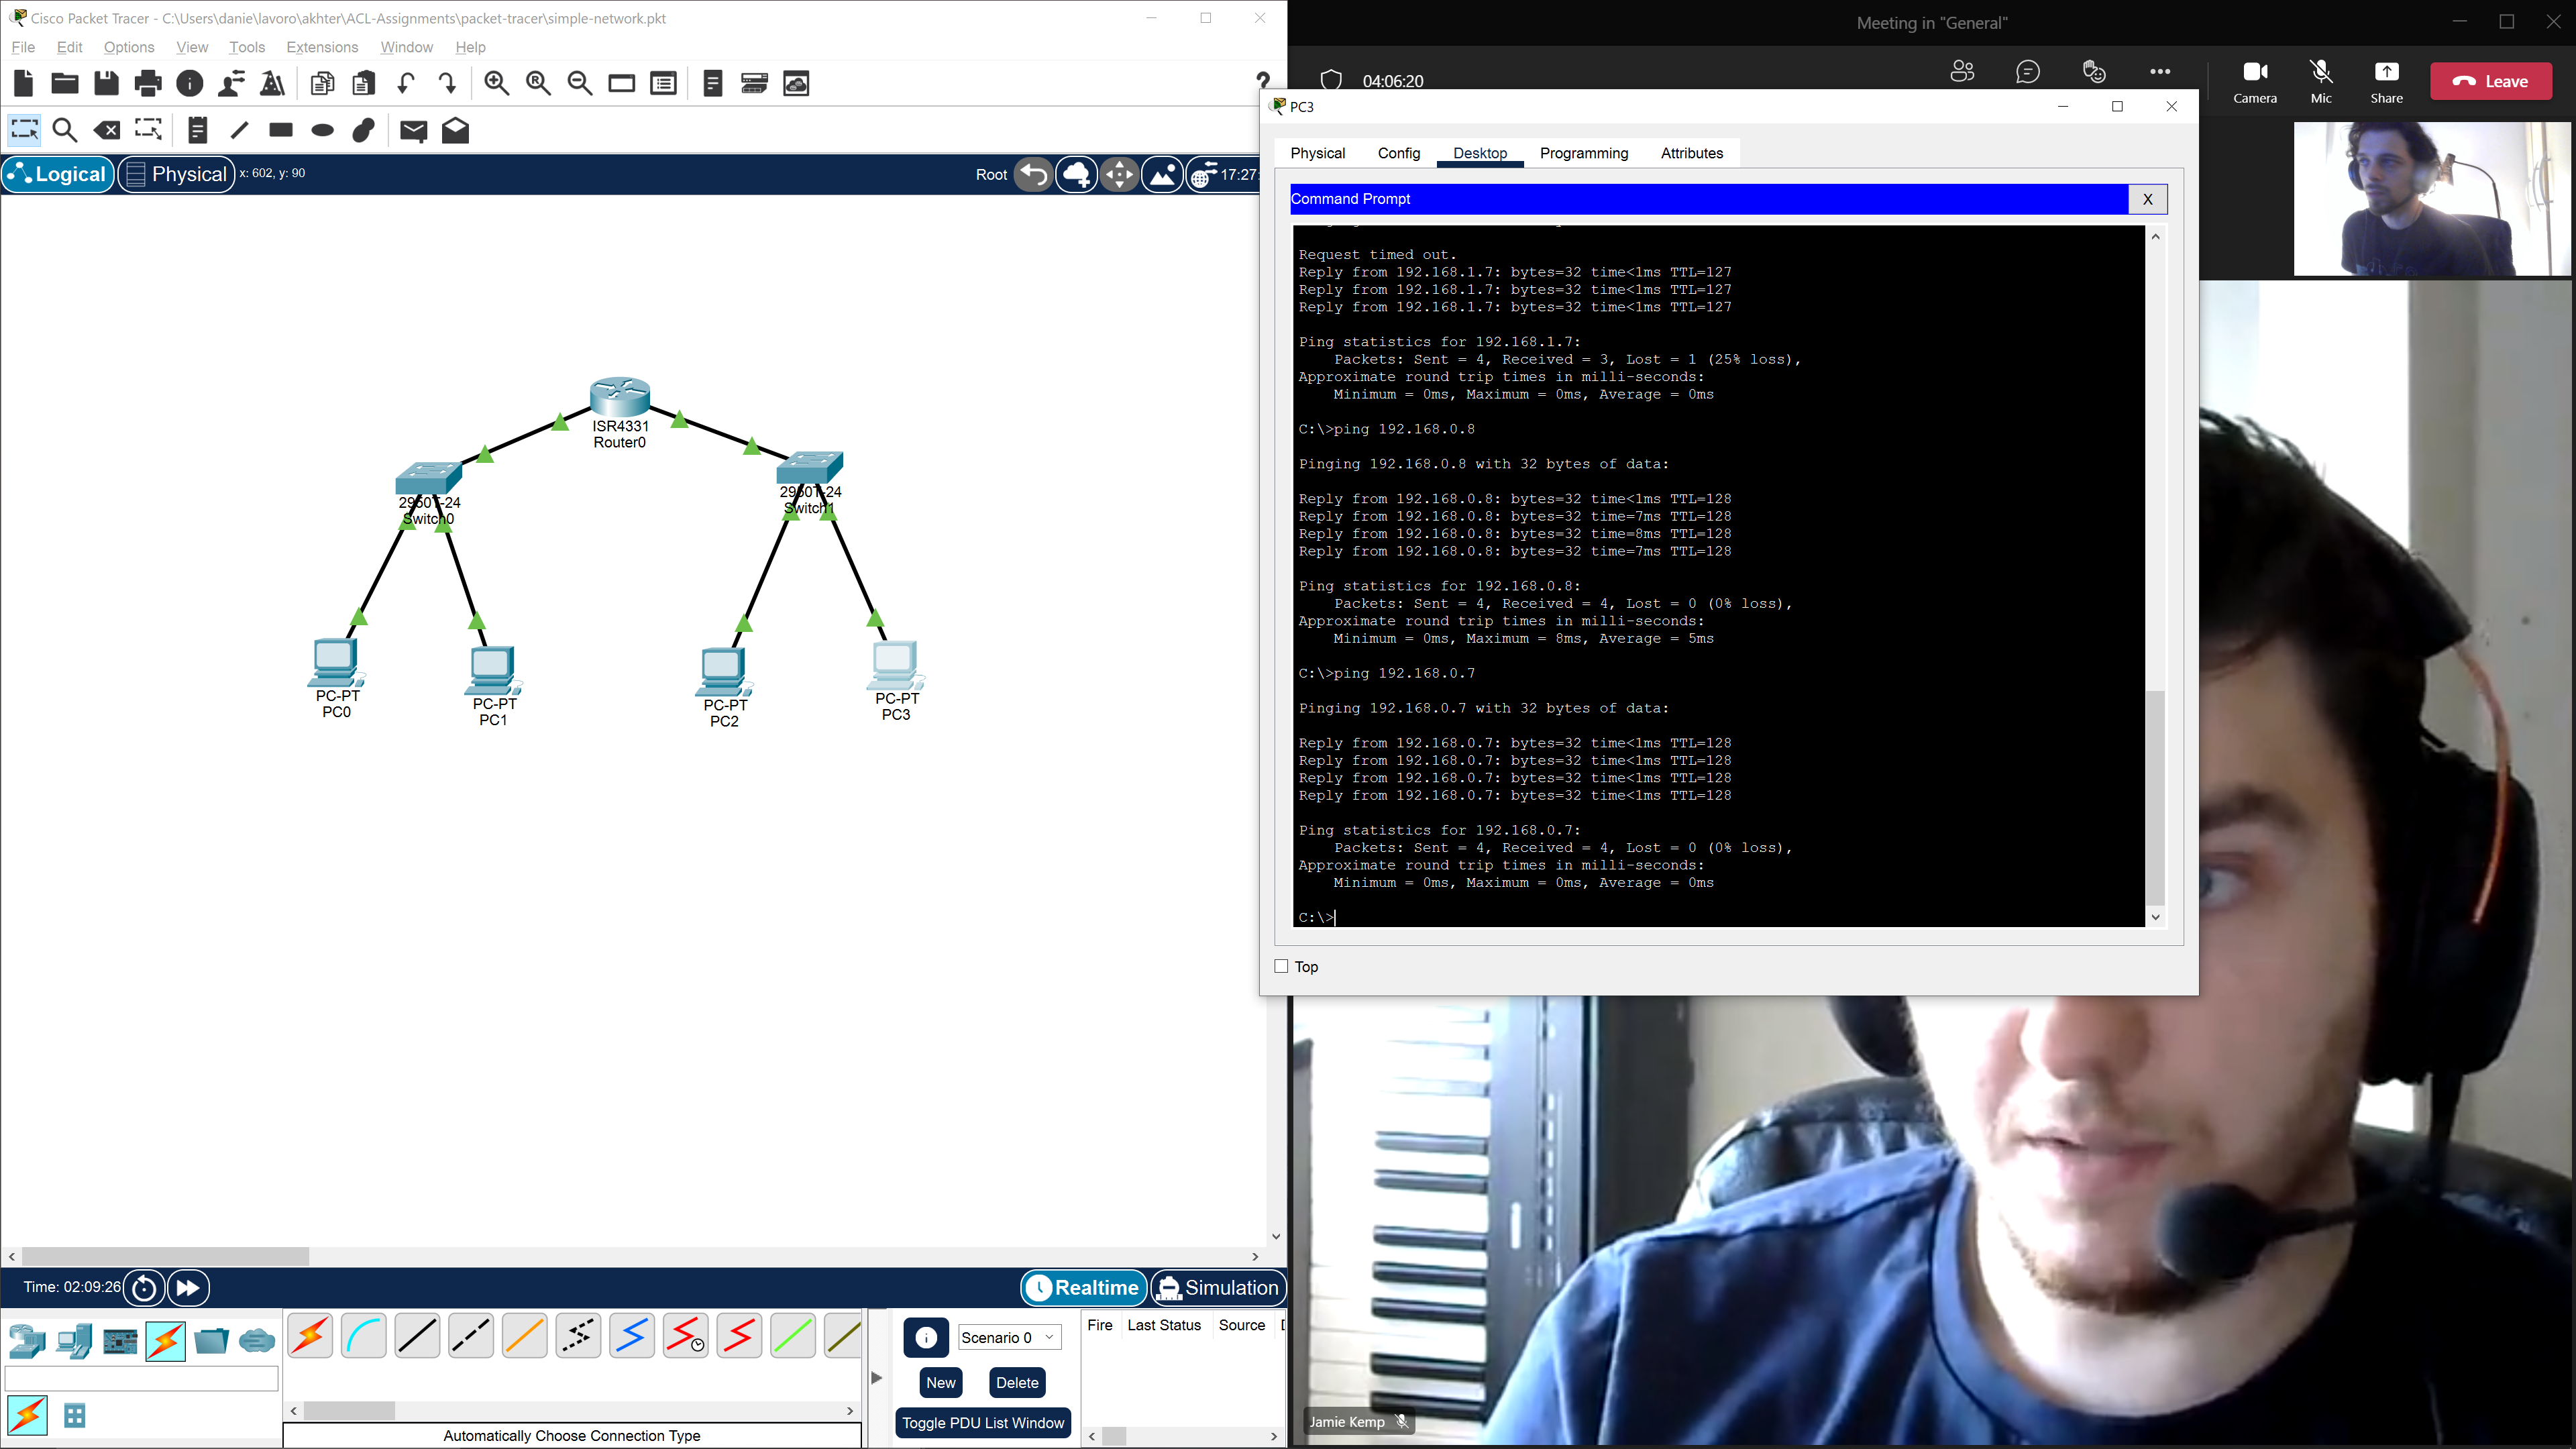
\includegraphics[width=9cm]{./ping.PNG}

\clearpage

\subsection{A step-by-step guide}

The following is what we've got when we open Cisco Packet Tracer : \newline

\noindent 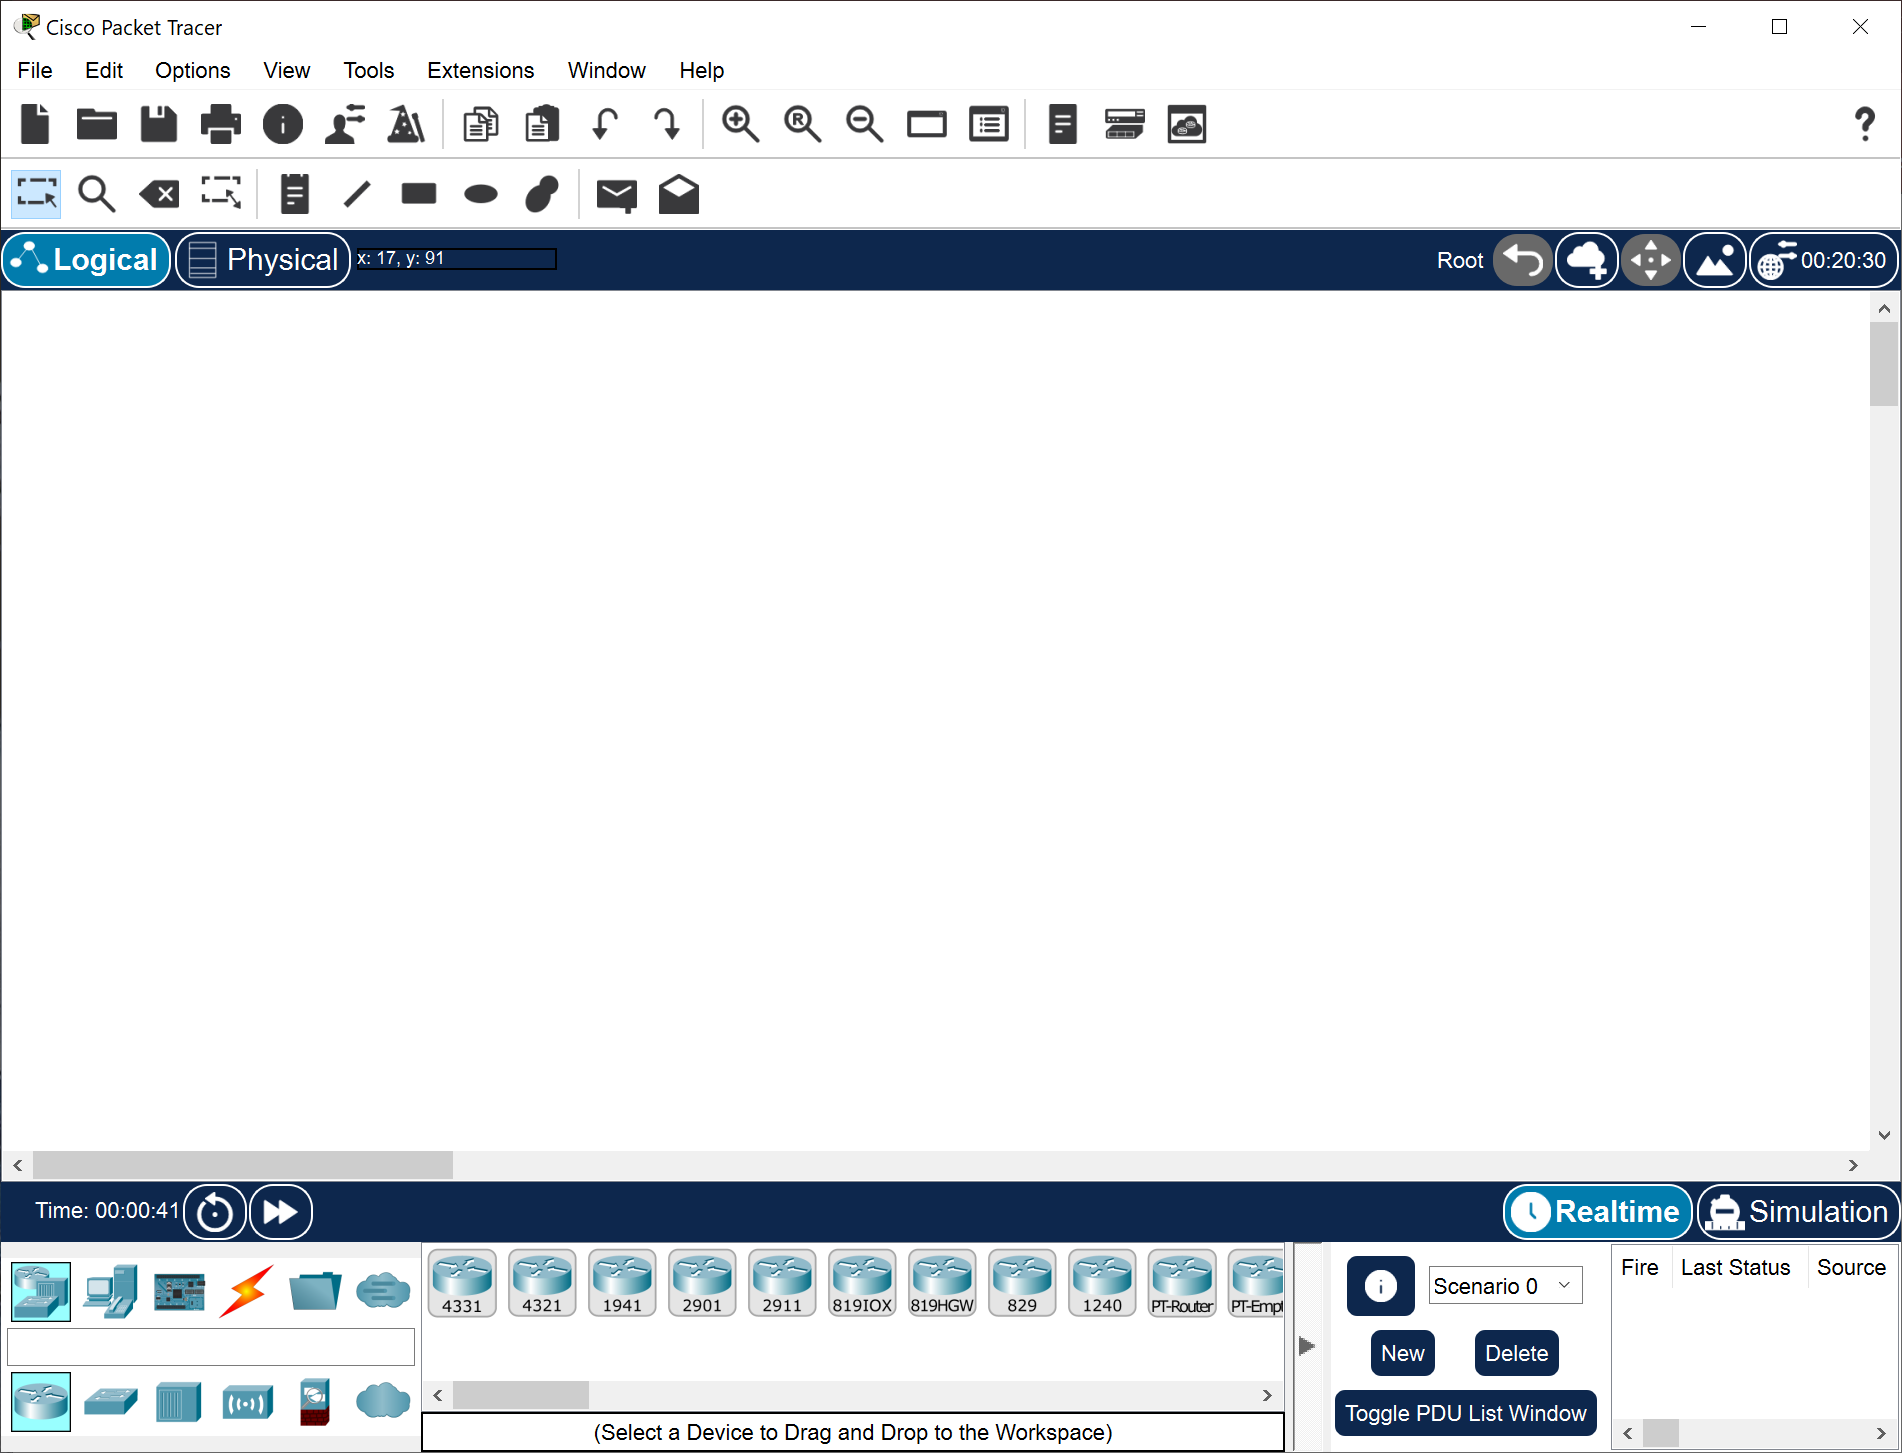
\includegraphics[width=13cm]{./step-by-step/0.PNG}
\clearpage

\noindent Now we add a switch : \newline

\noindent 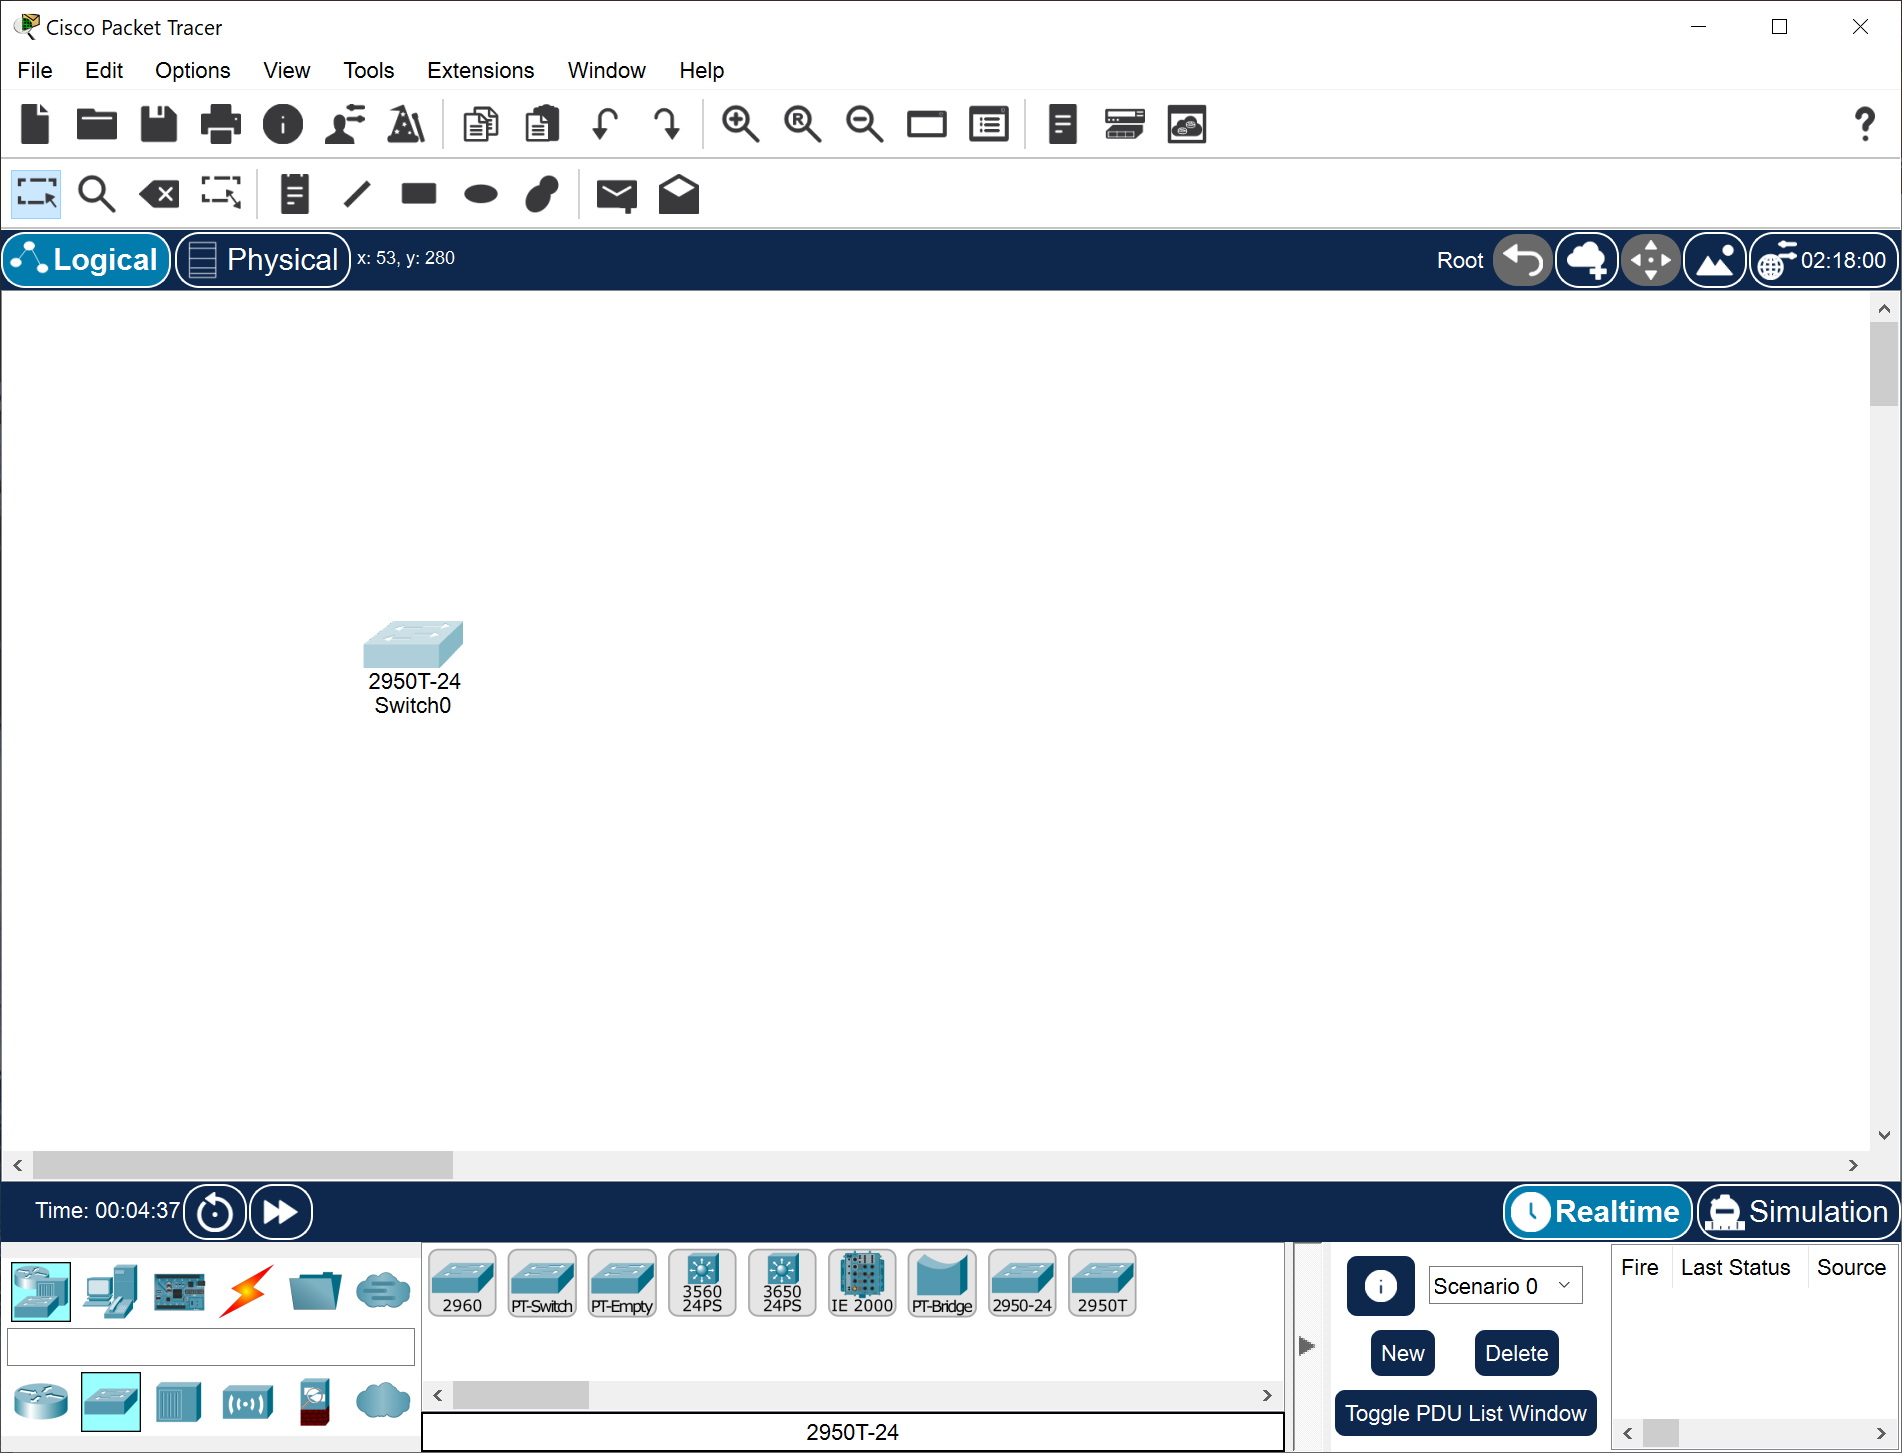
\includegraphics[width=13cm]{./step-by-step/1.PNG}
\clearpage

\noindent Now we add a computer : \newline

\noindent 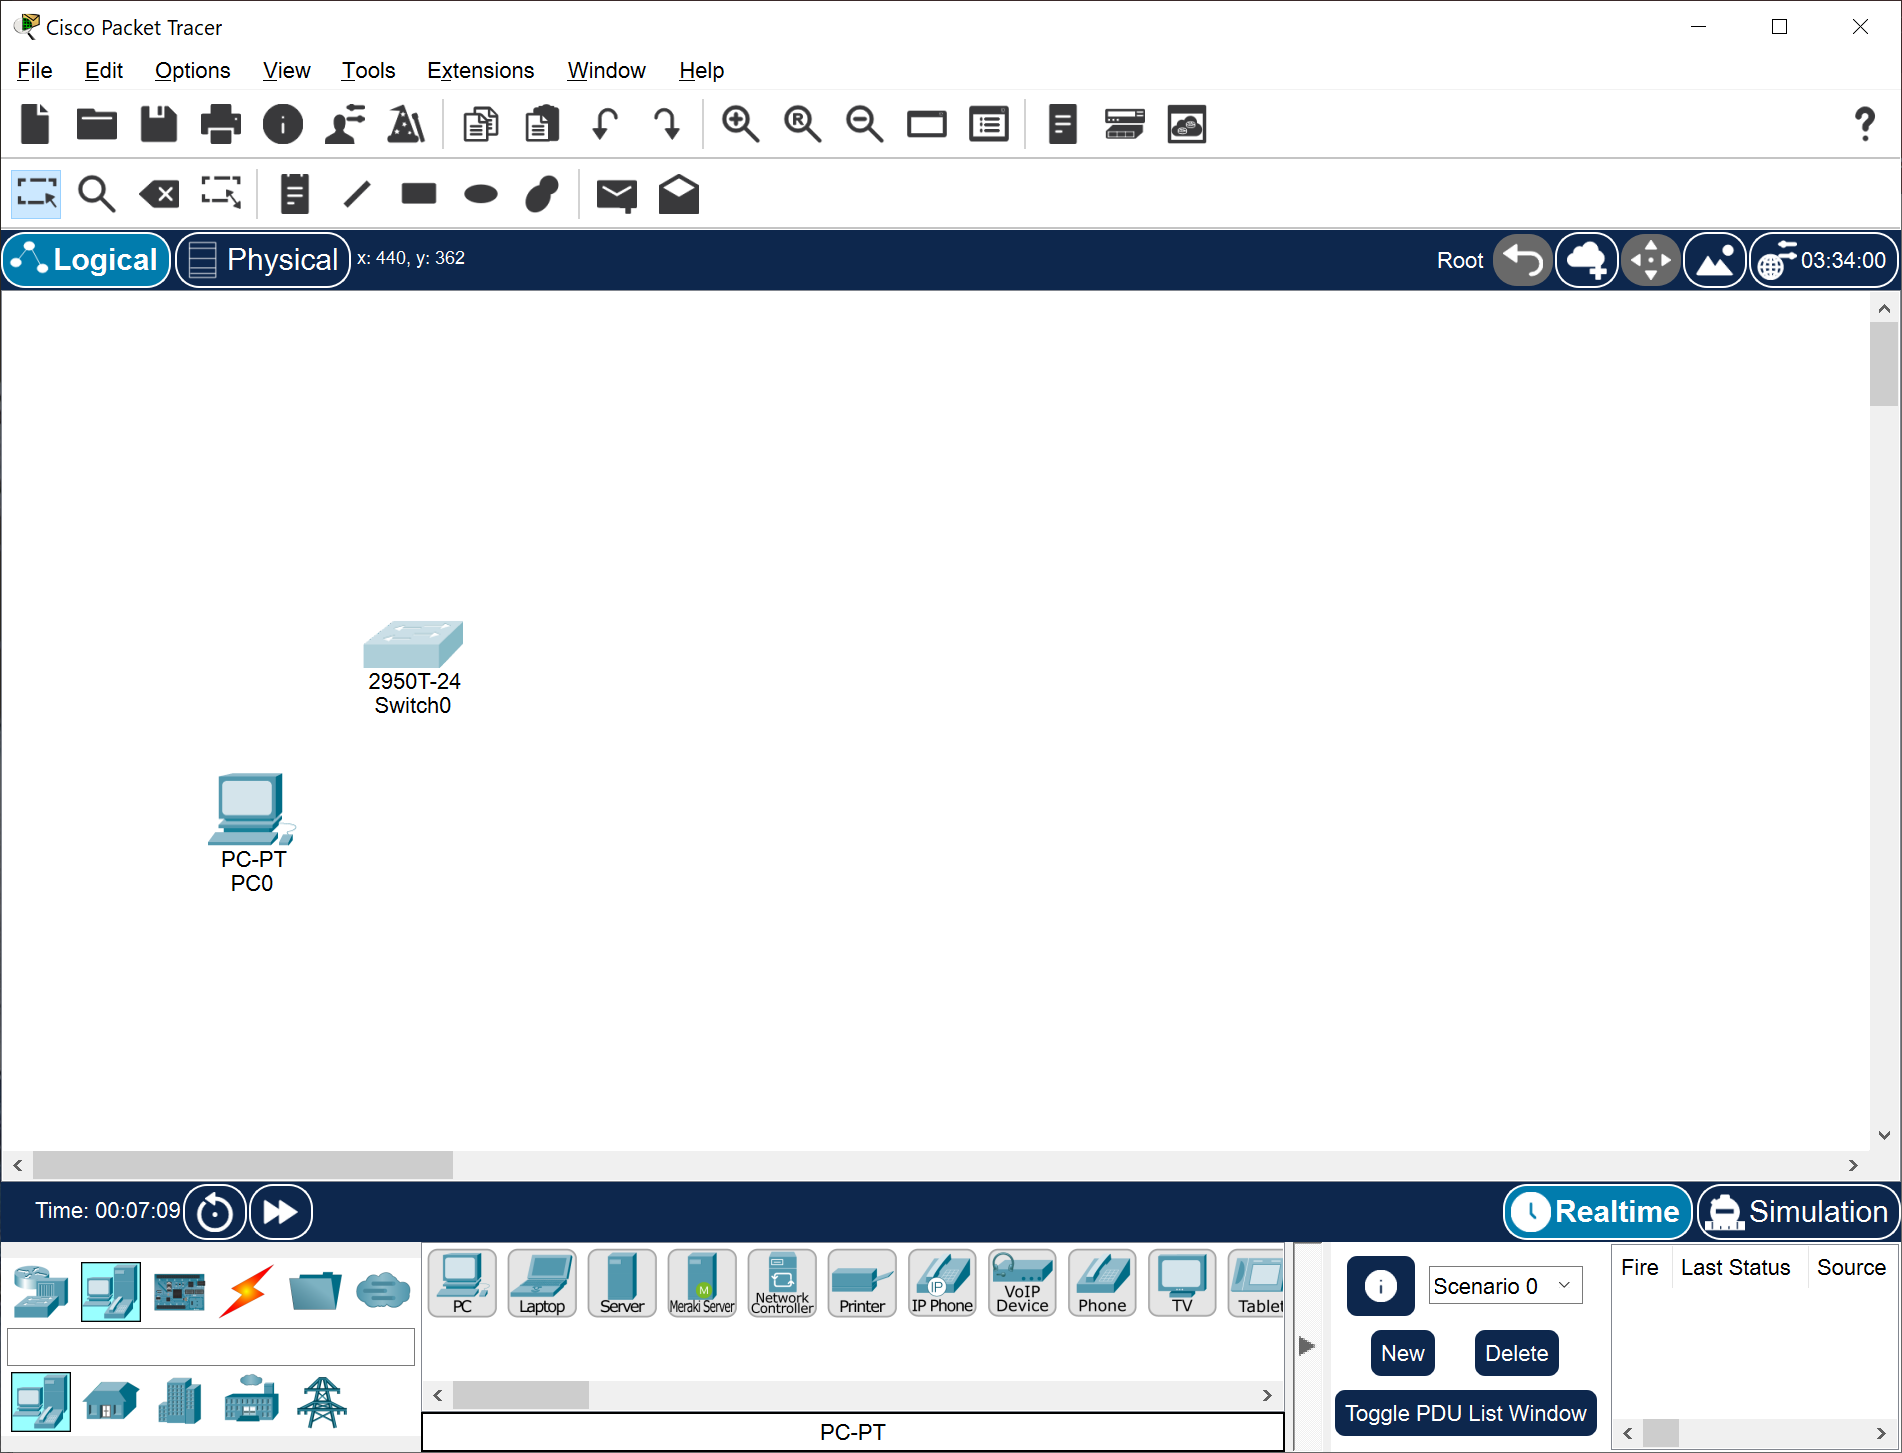
\includegraphics[width=13cm]{./step-by-step/2.PNG}
\clearpage

\noindent Now we click on the computer \newline

\noindent 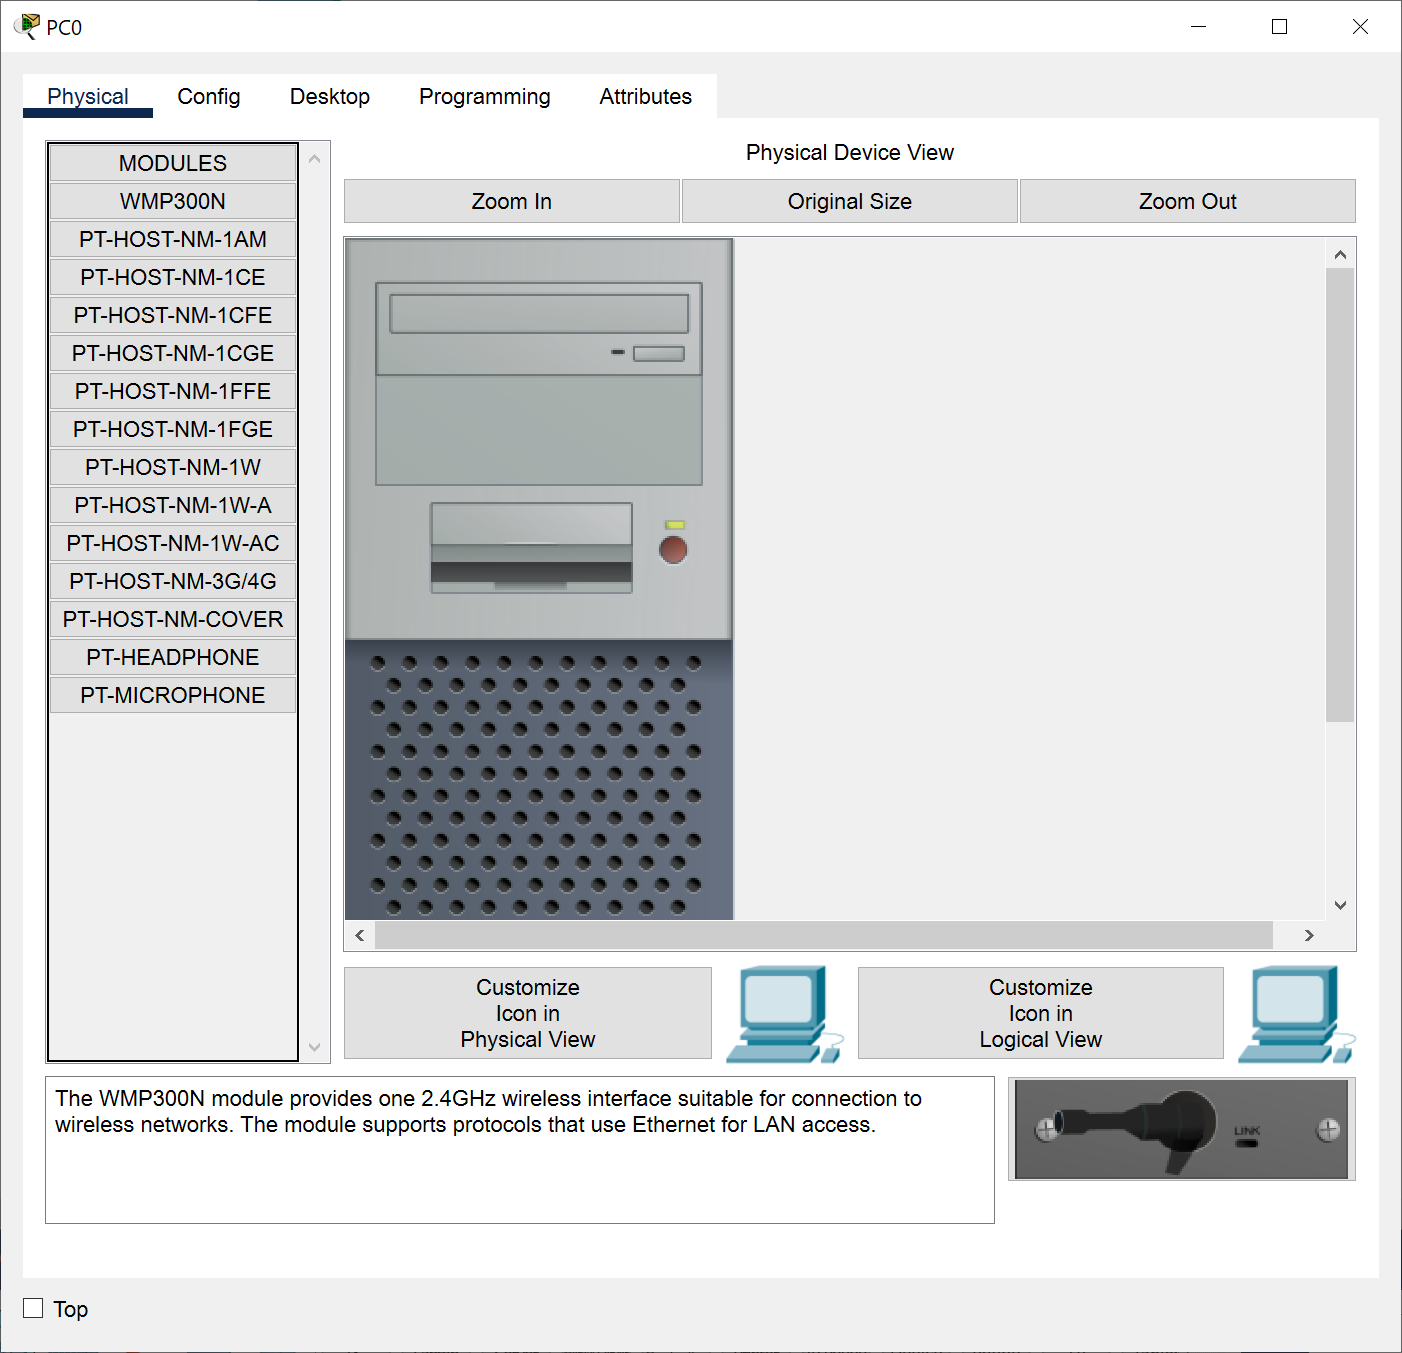
\includegraphics[width=13cm]{./step-by-step/3.PNG}
\clearpage

\noindent And we move ourselves in the \textvg{Config} tab \newline

\noindent 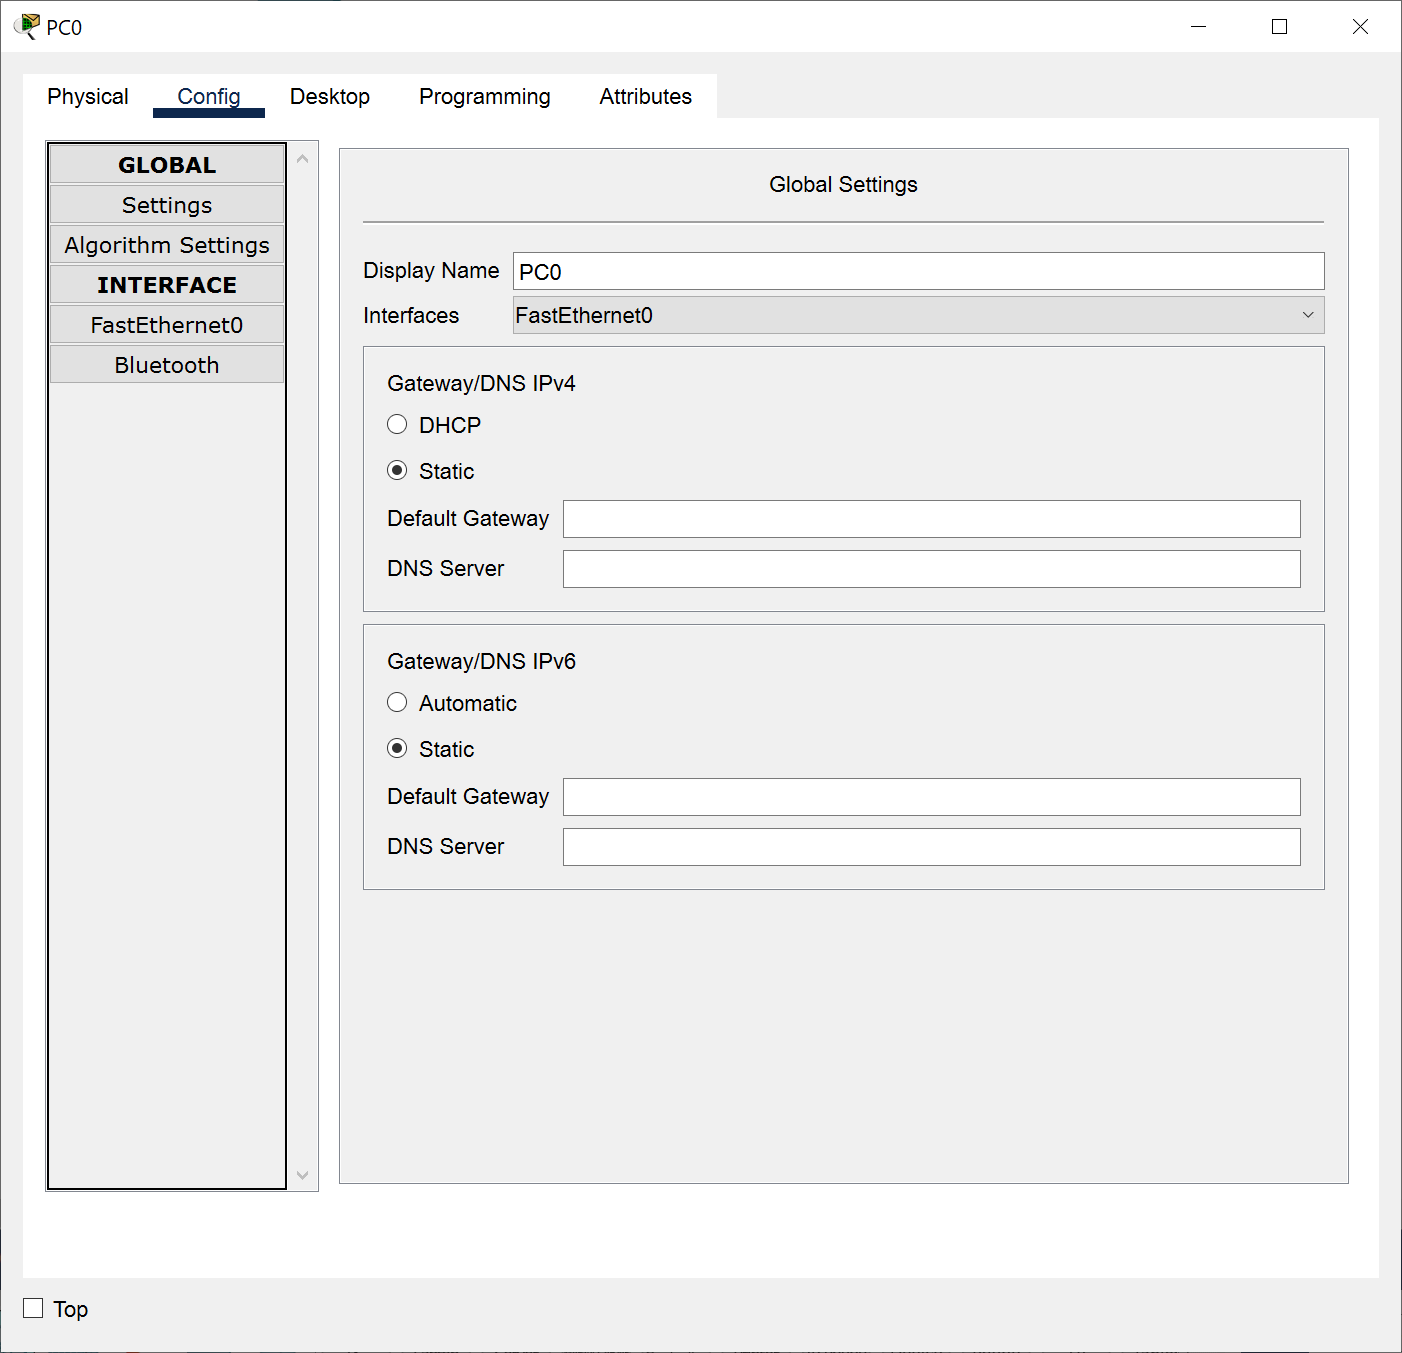
\includegraphics[width=13cm]{./step-by-step/4.PNG}
\clearpage

\noindent what we're gonna be looking later at is the IPV4 address \newline

\noindent 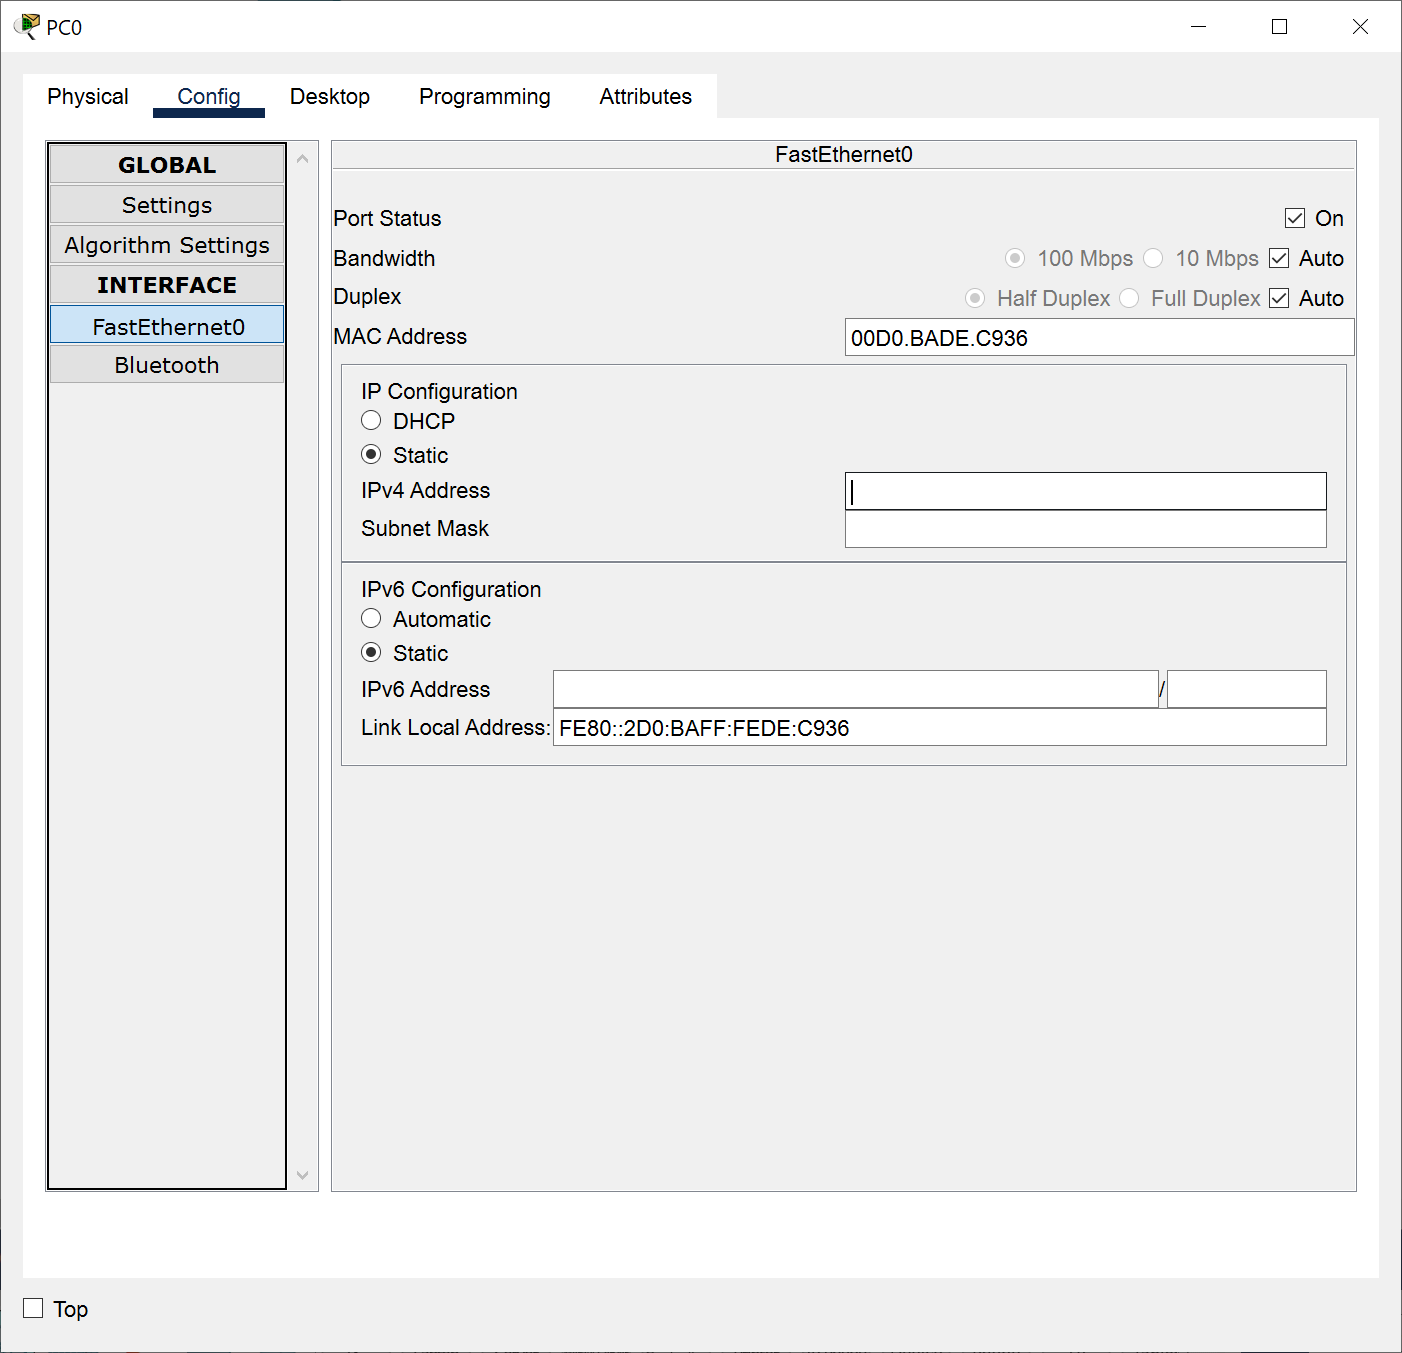
\includegraphics[width=13cm]{./step-by-step/5.PNG}
\clearpage

\noindent in the meantime let's  go in global and set the \textbf{IP Address} equal to this 

\[192.168.0.1\]

\noindent 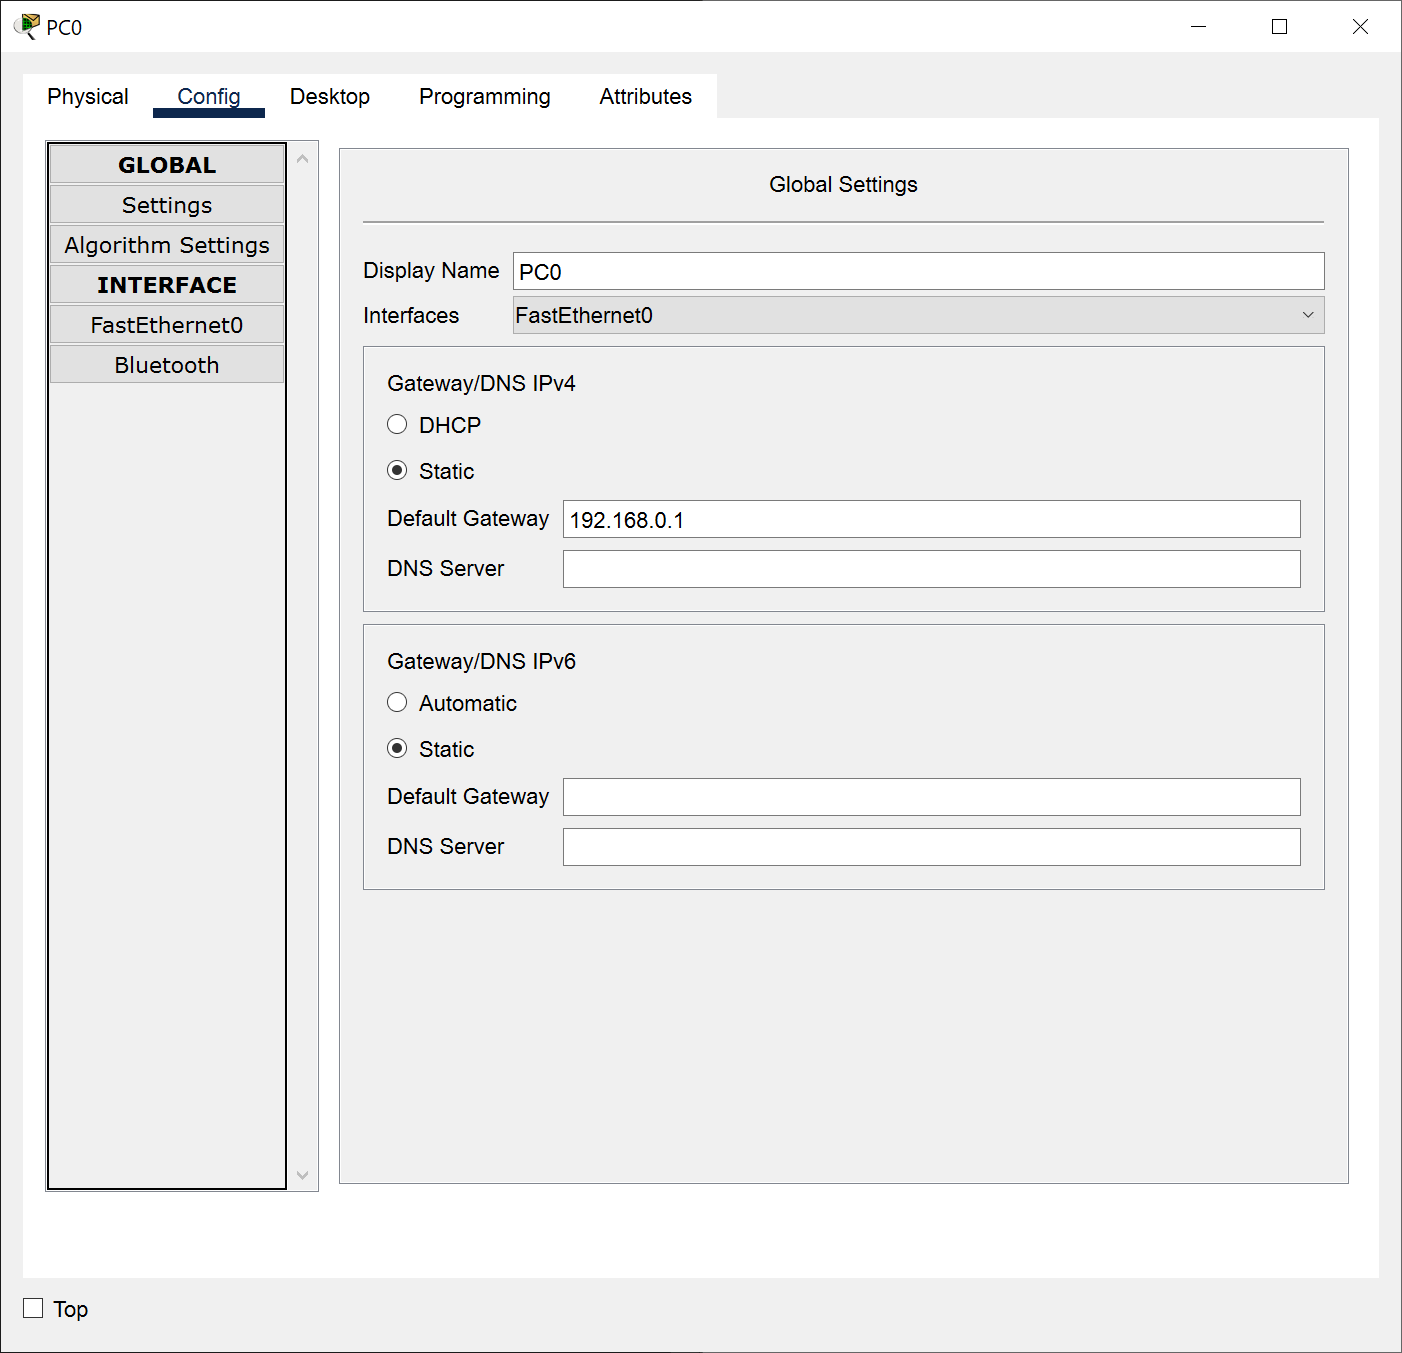
\includegraphics[width=13cm]{./step-by-step/6.PNG}
\clearpage

\noindent Now we add a new computer \newline

\noindent 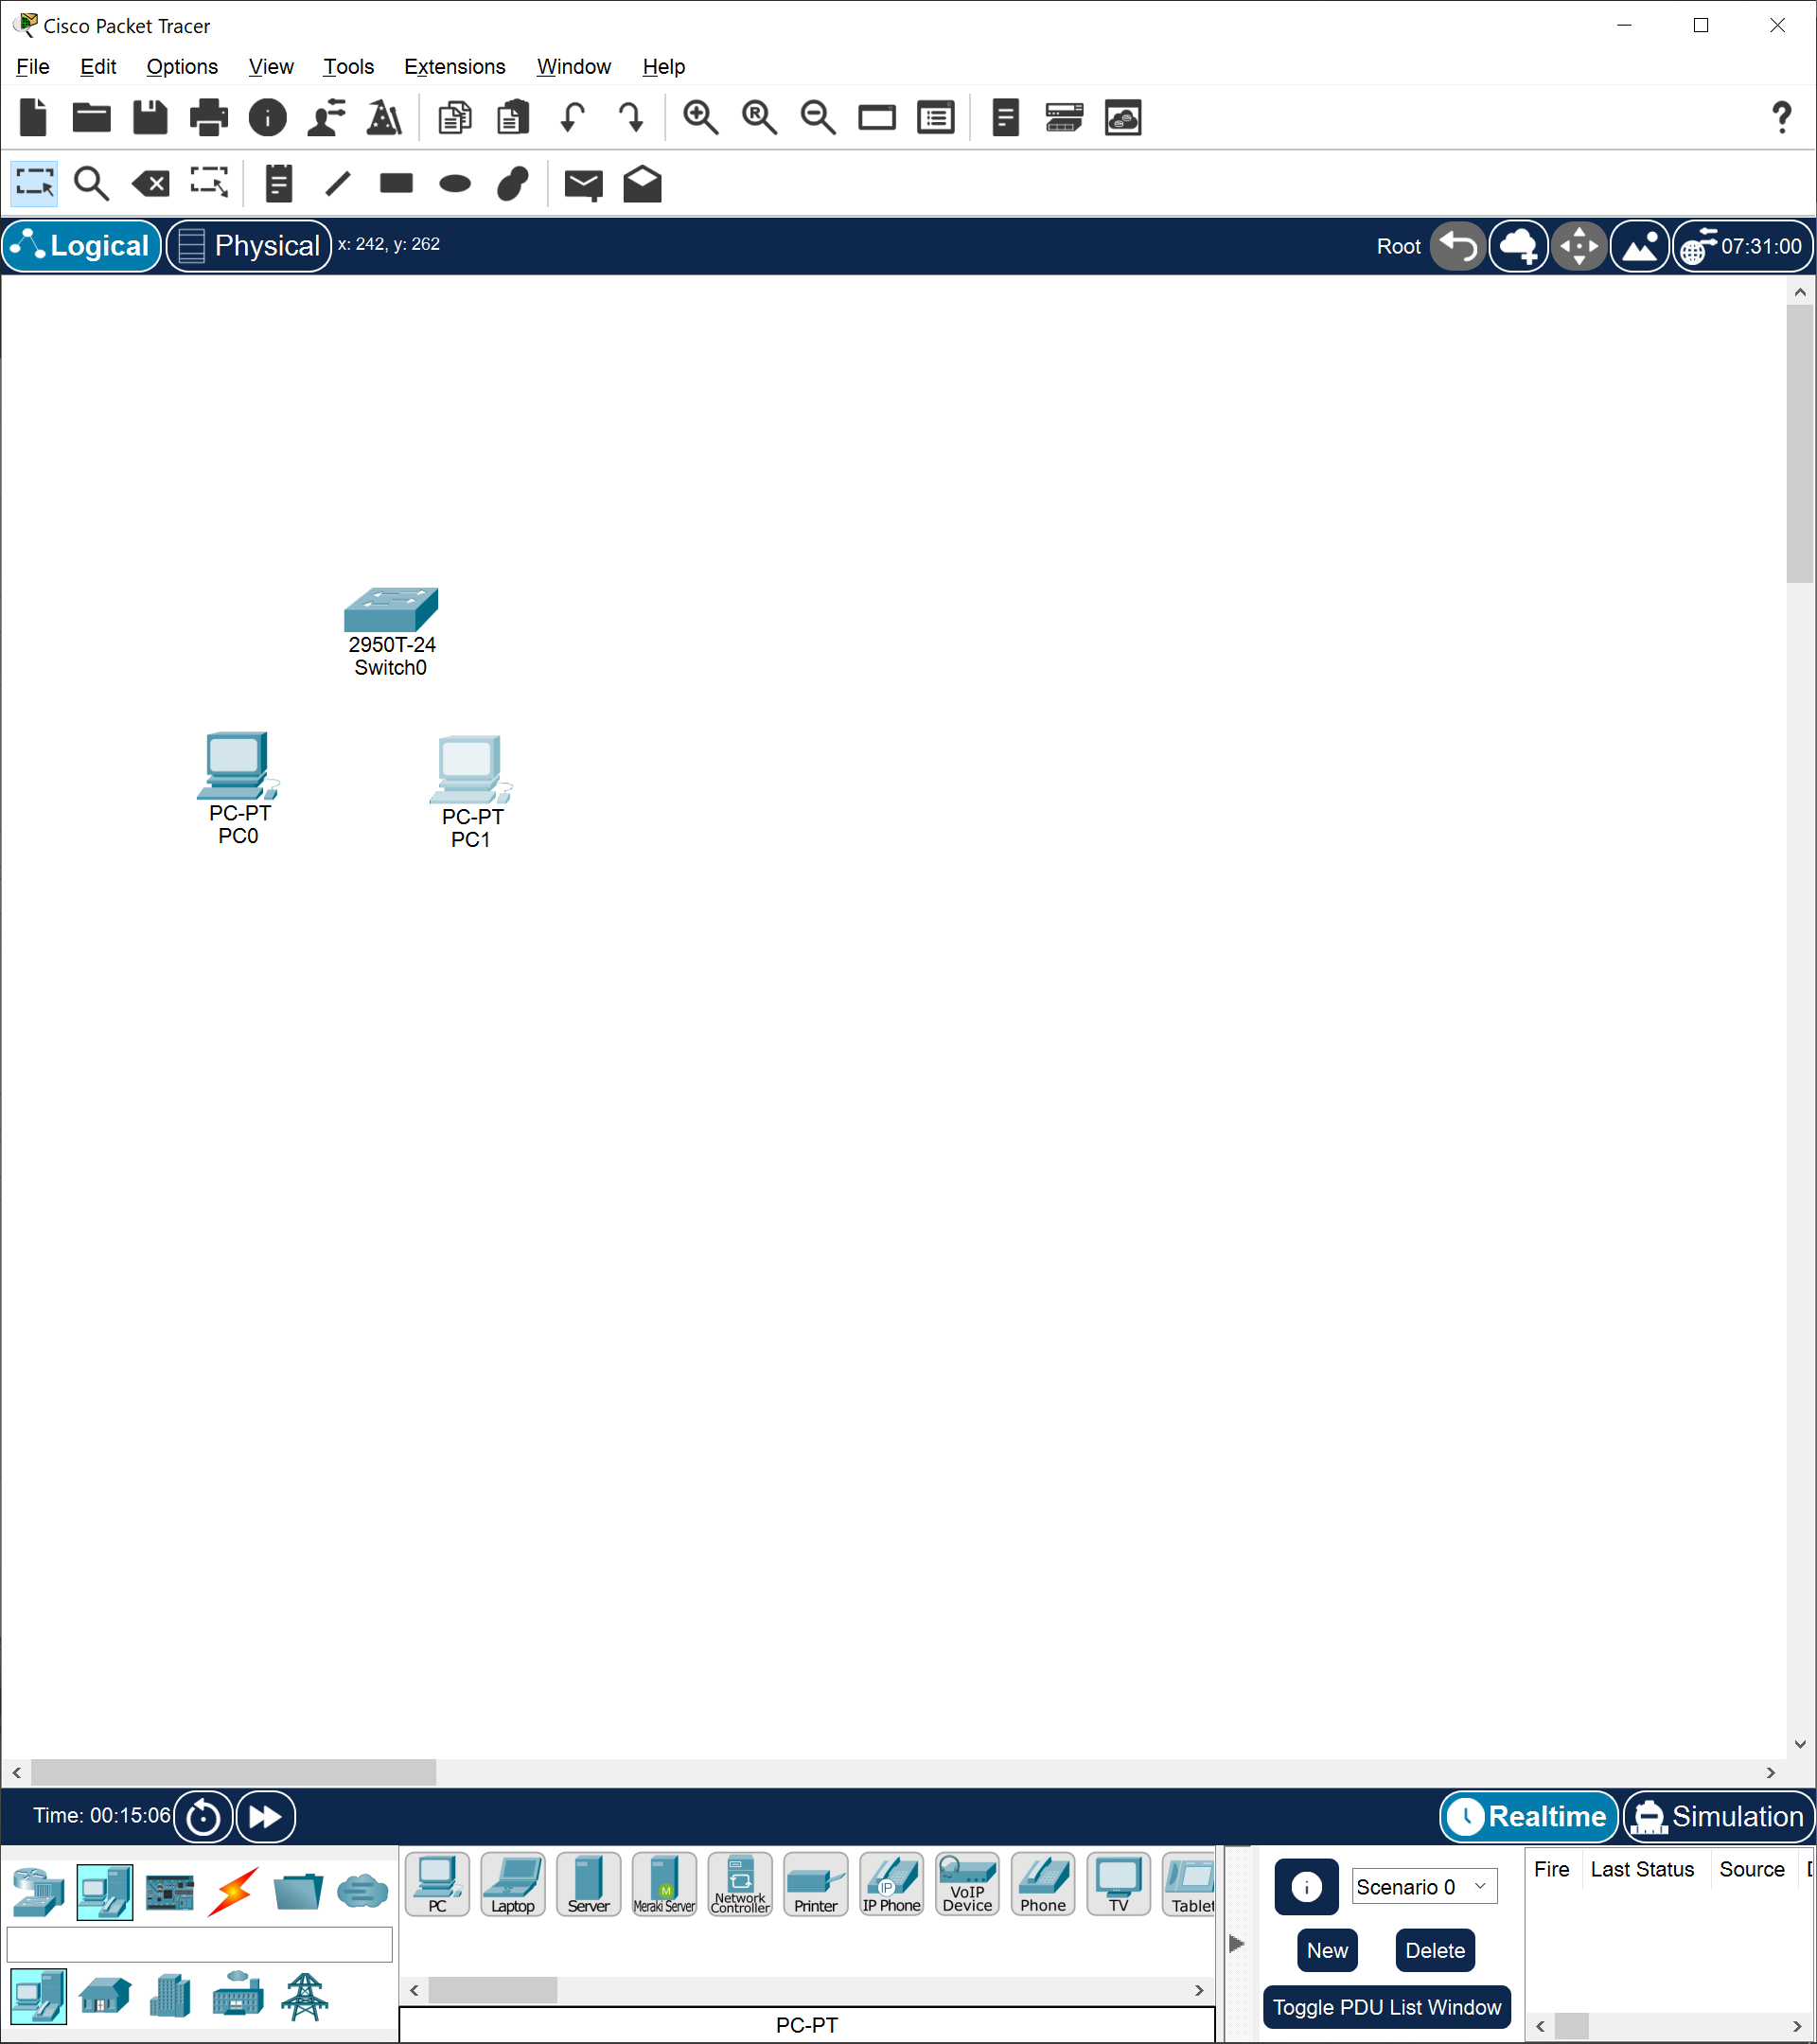
\includegraphics[width=13cm]{./step-by-step/7.PNG}
\clearpage


\noindent We link the switch to the first computer and wait for all lights to go green \newline

\noindent 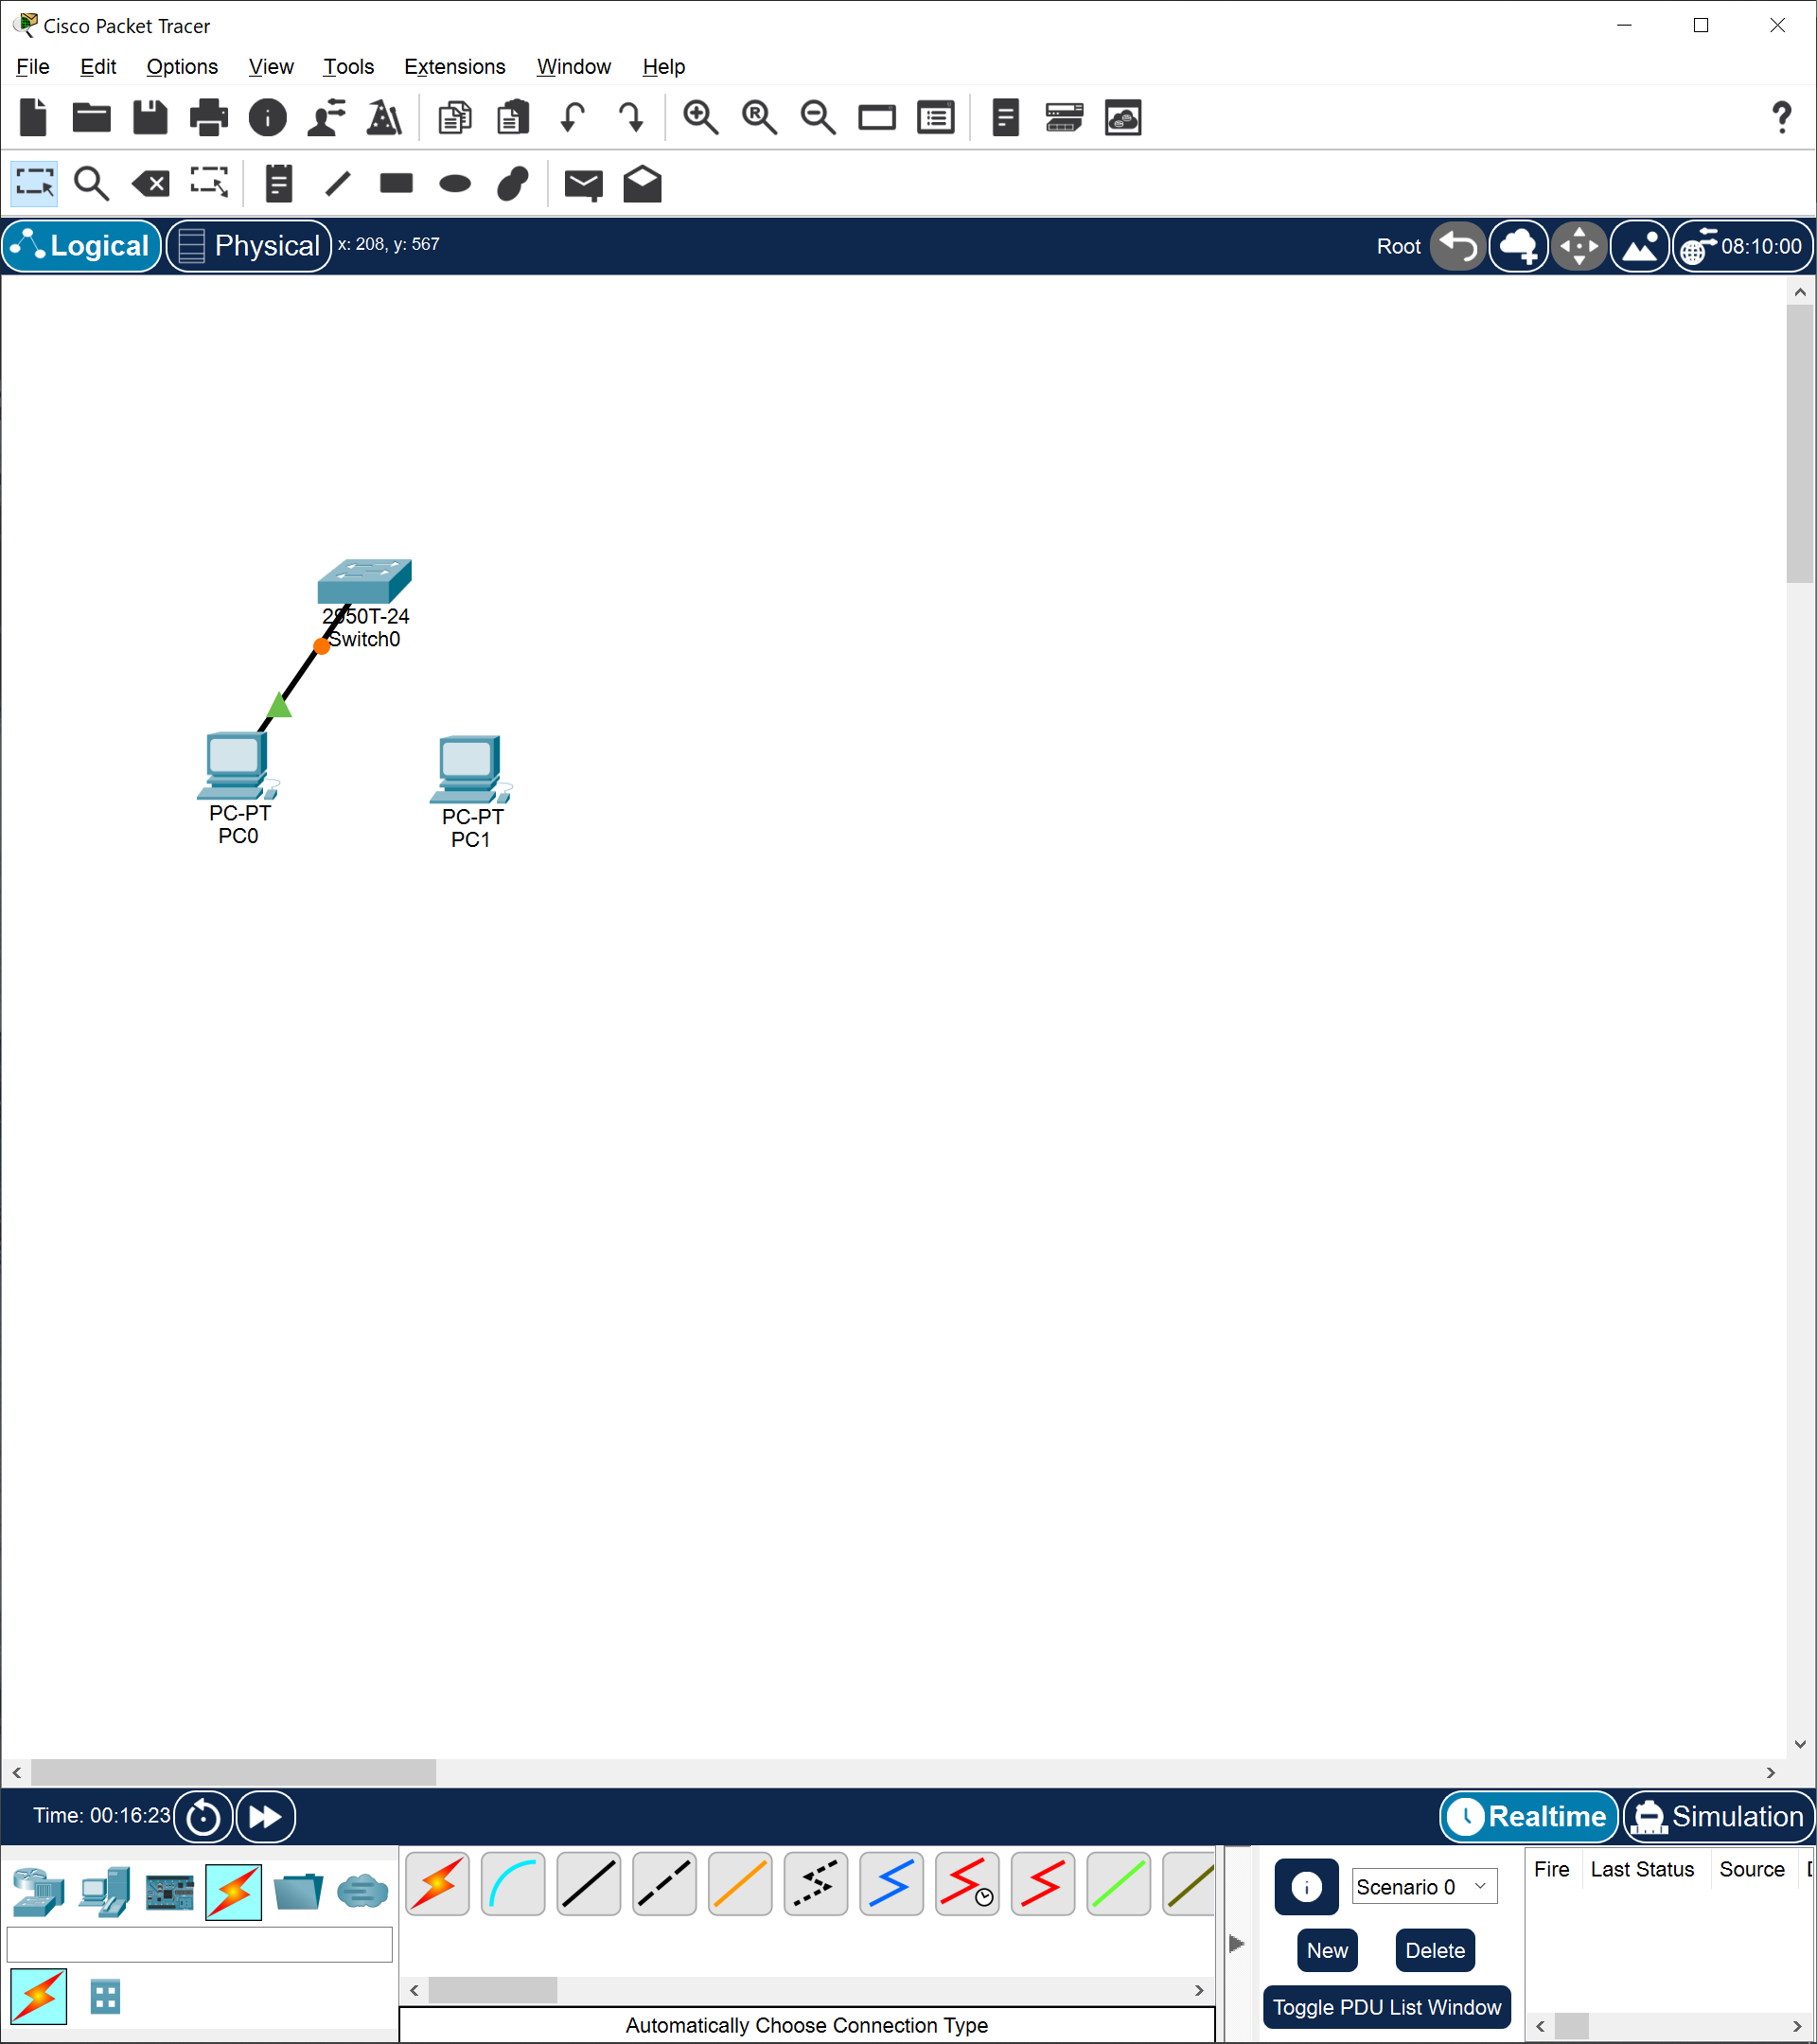
\includegraphics[width=13cm]{./step-by-step/8.PNG}
\clearpage

\noindent Link the switch to the second computer and wait for this link to go all green as well \newline

\noindent 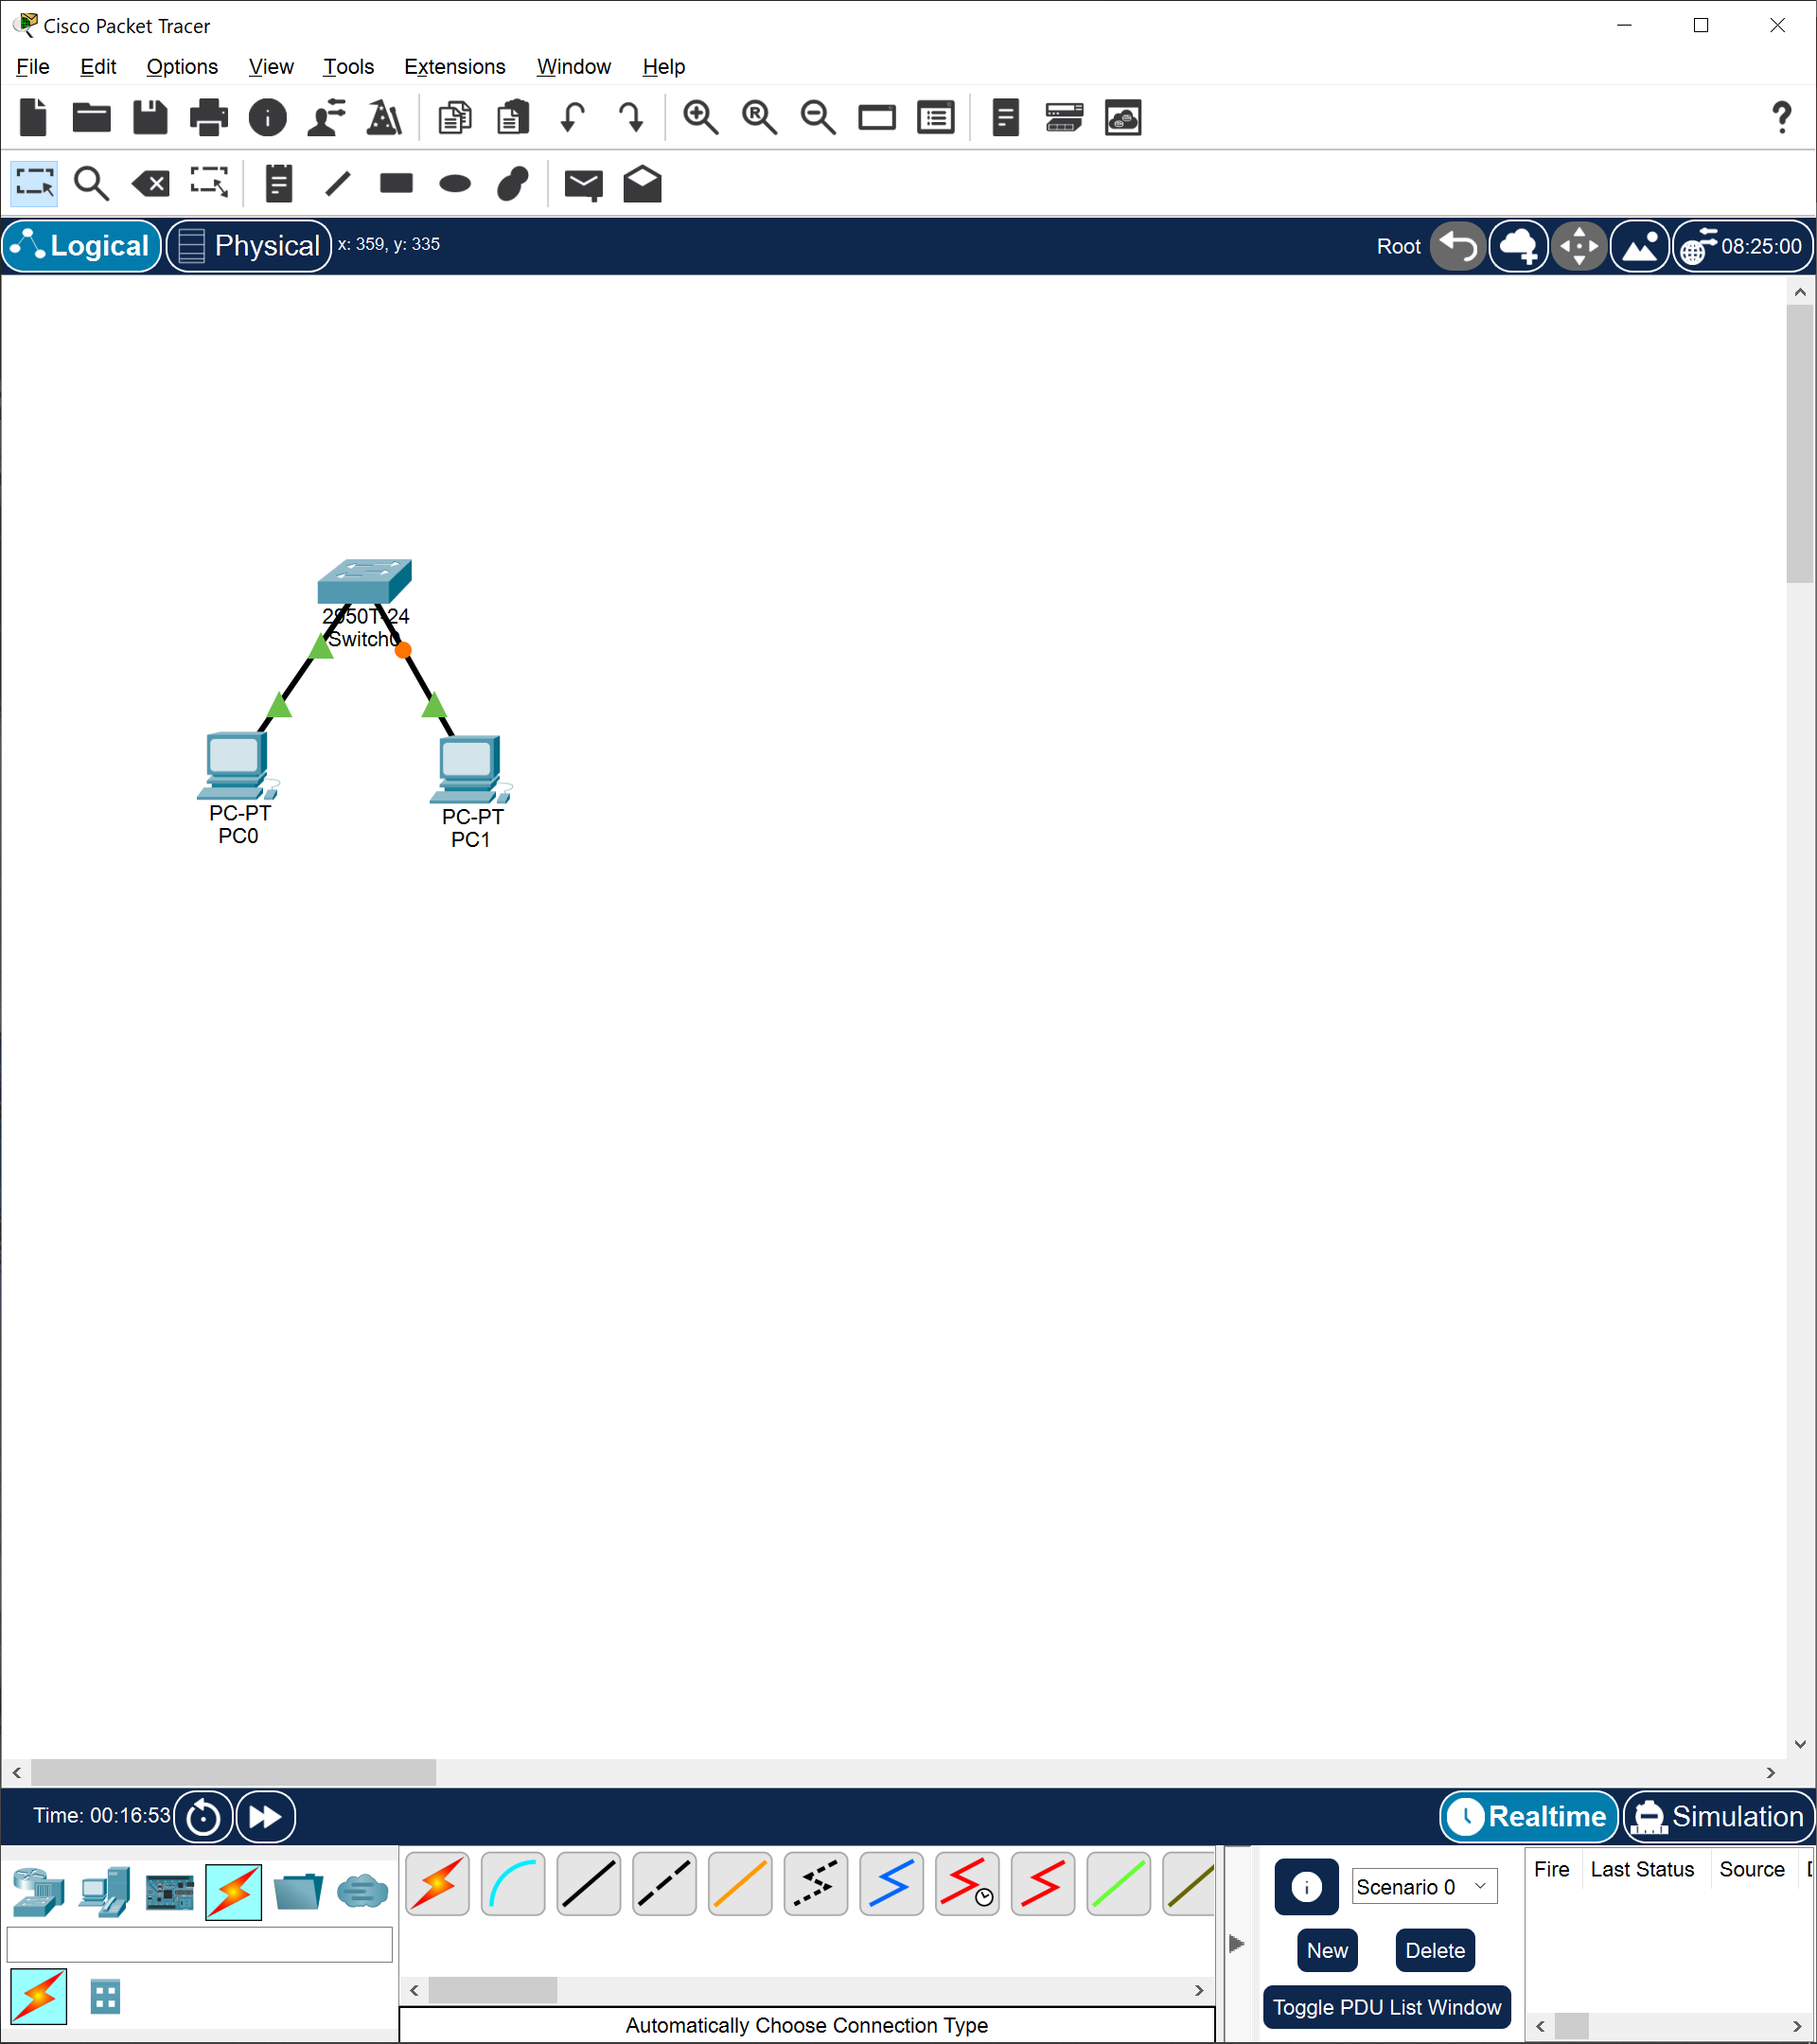
\includegraphics[width=13cm]{./step-by-step/9.PNG}
\clearpage

\noindent Now it's all green which makes us happy \newline

\noindent 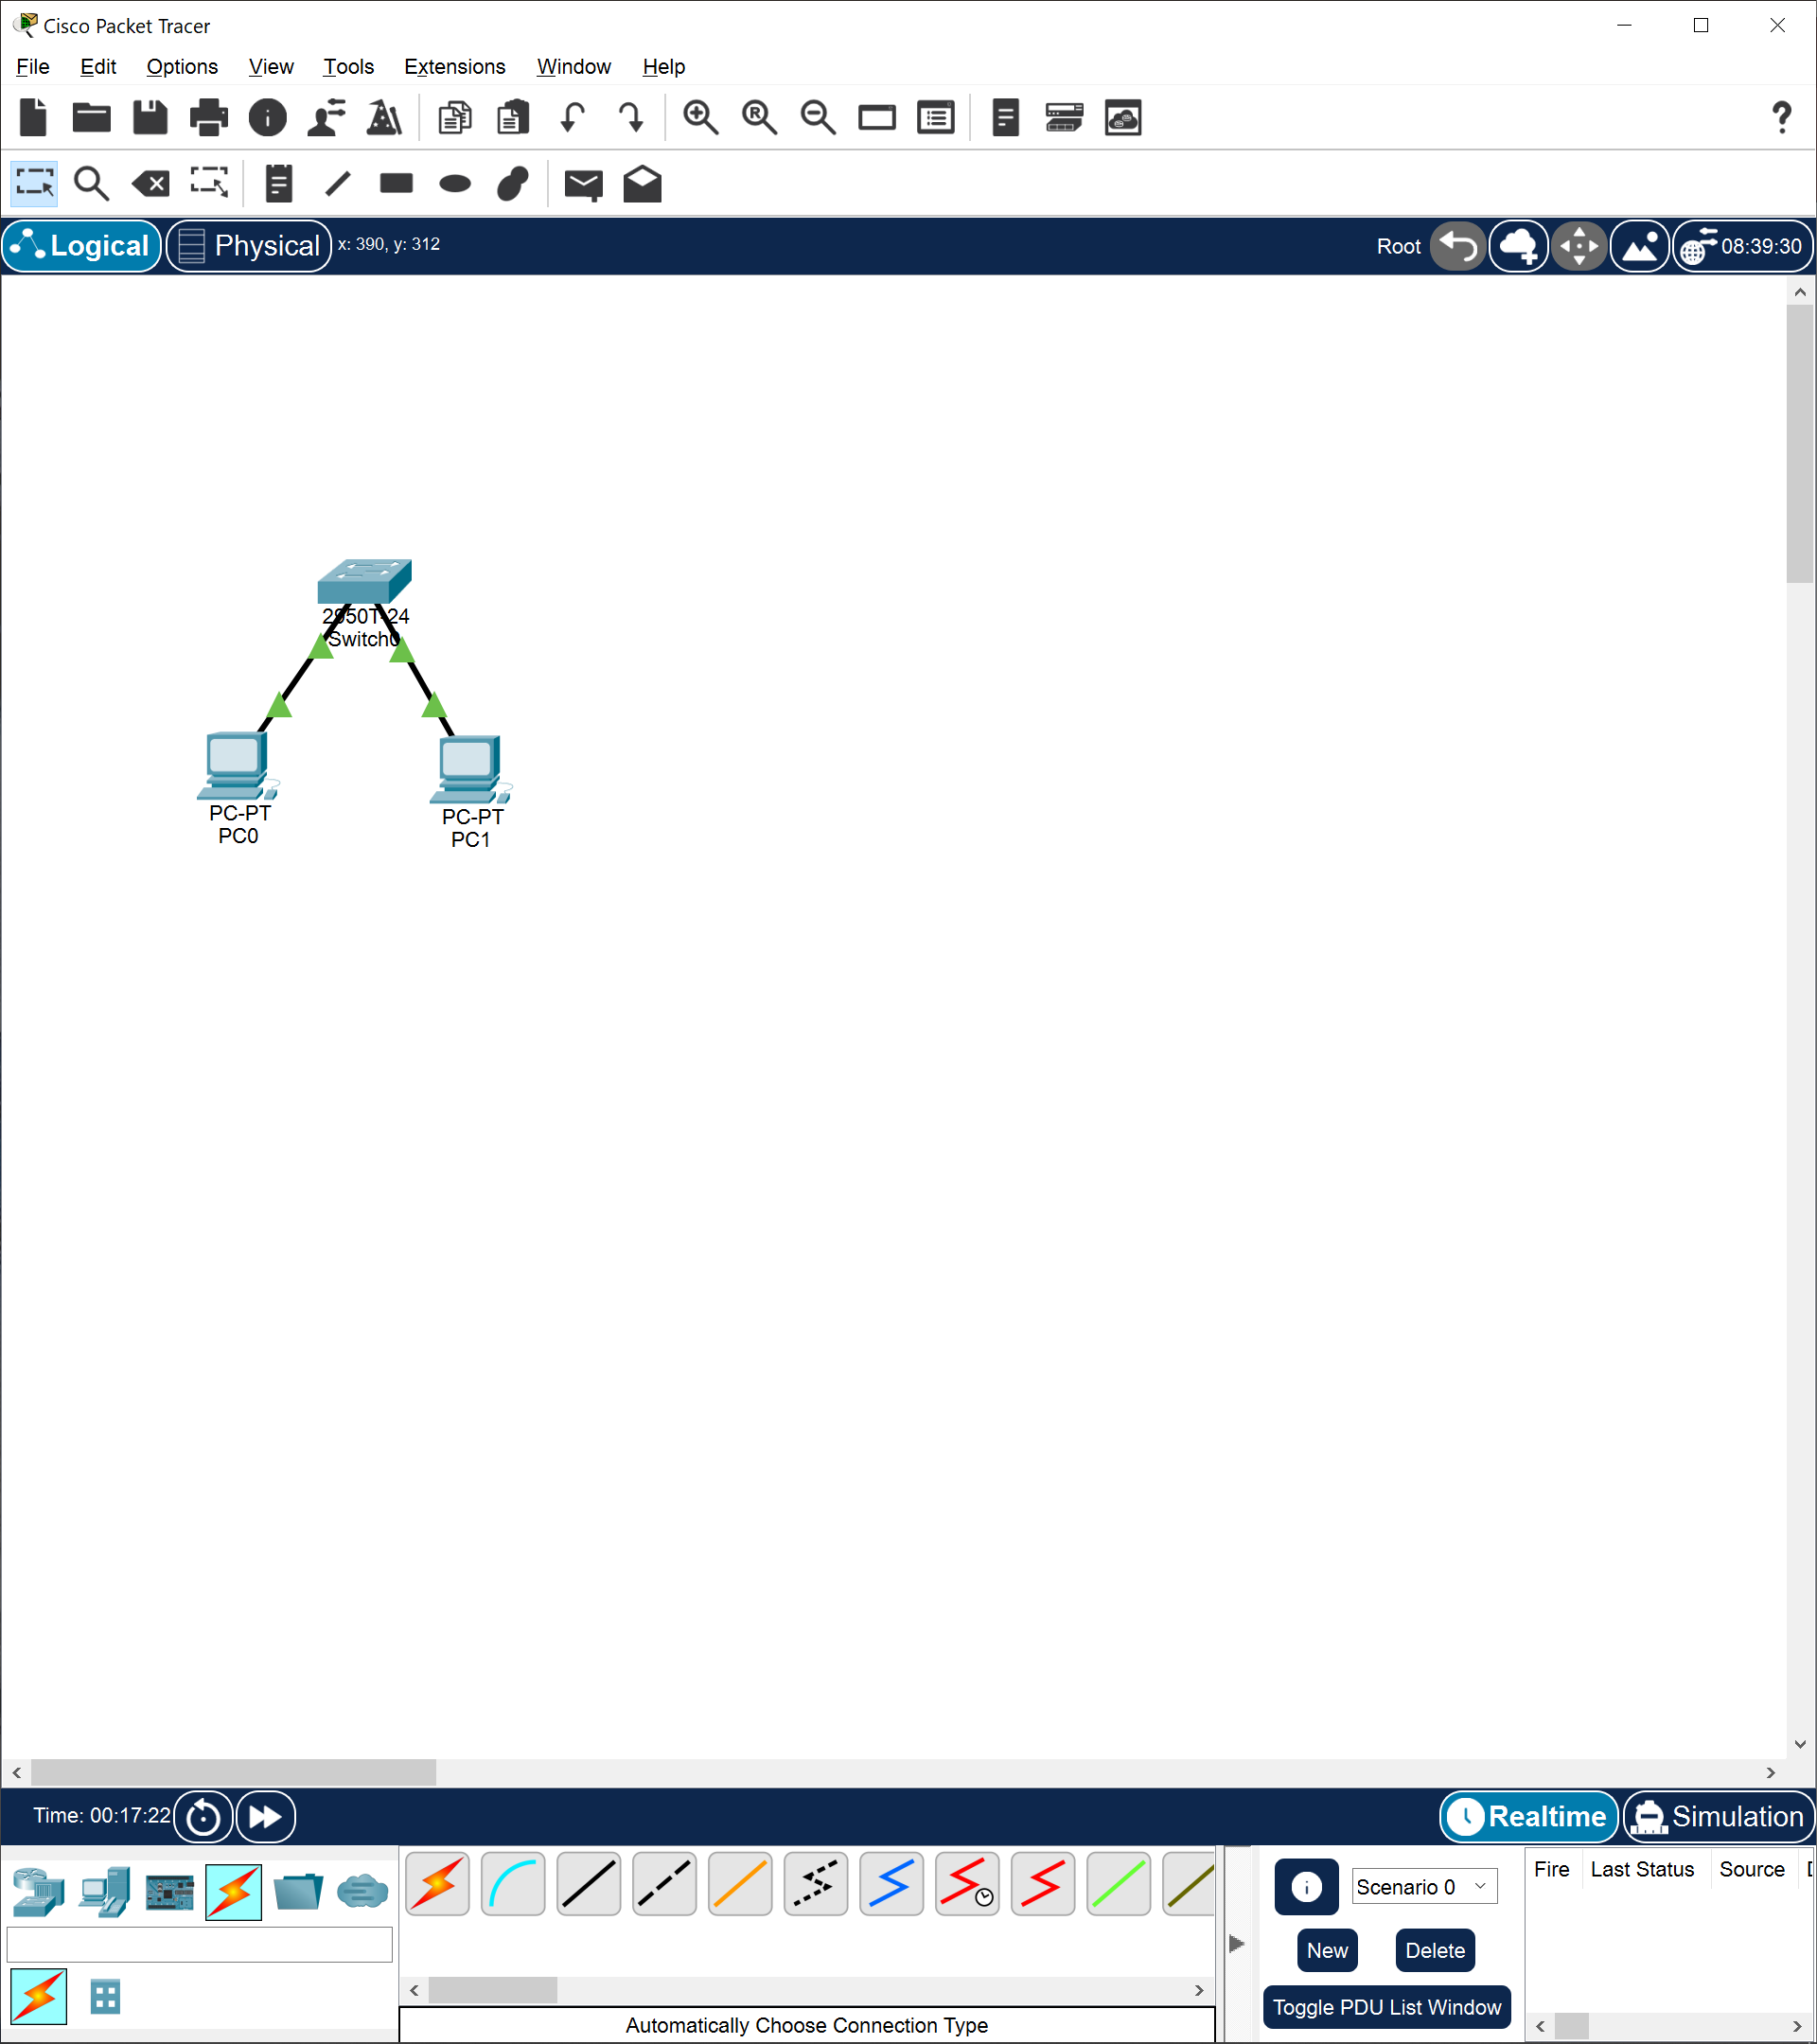
\includegraphics[width=13cm]{./step-by-step/10.PNG}
\clearpage

\noindent Let's add a router \newline

\noindent 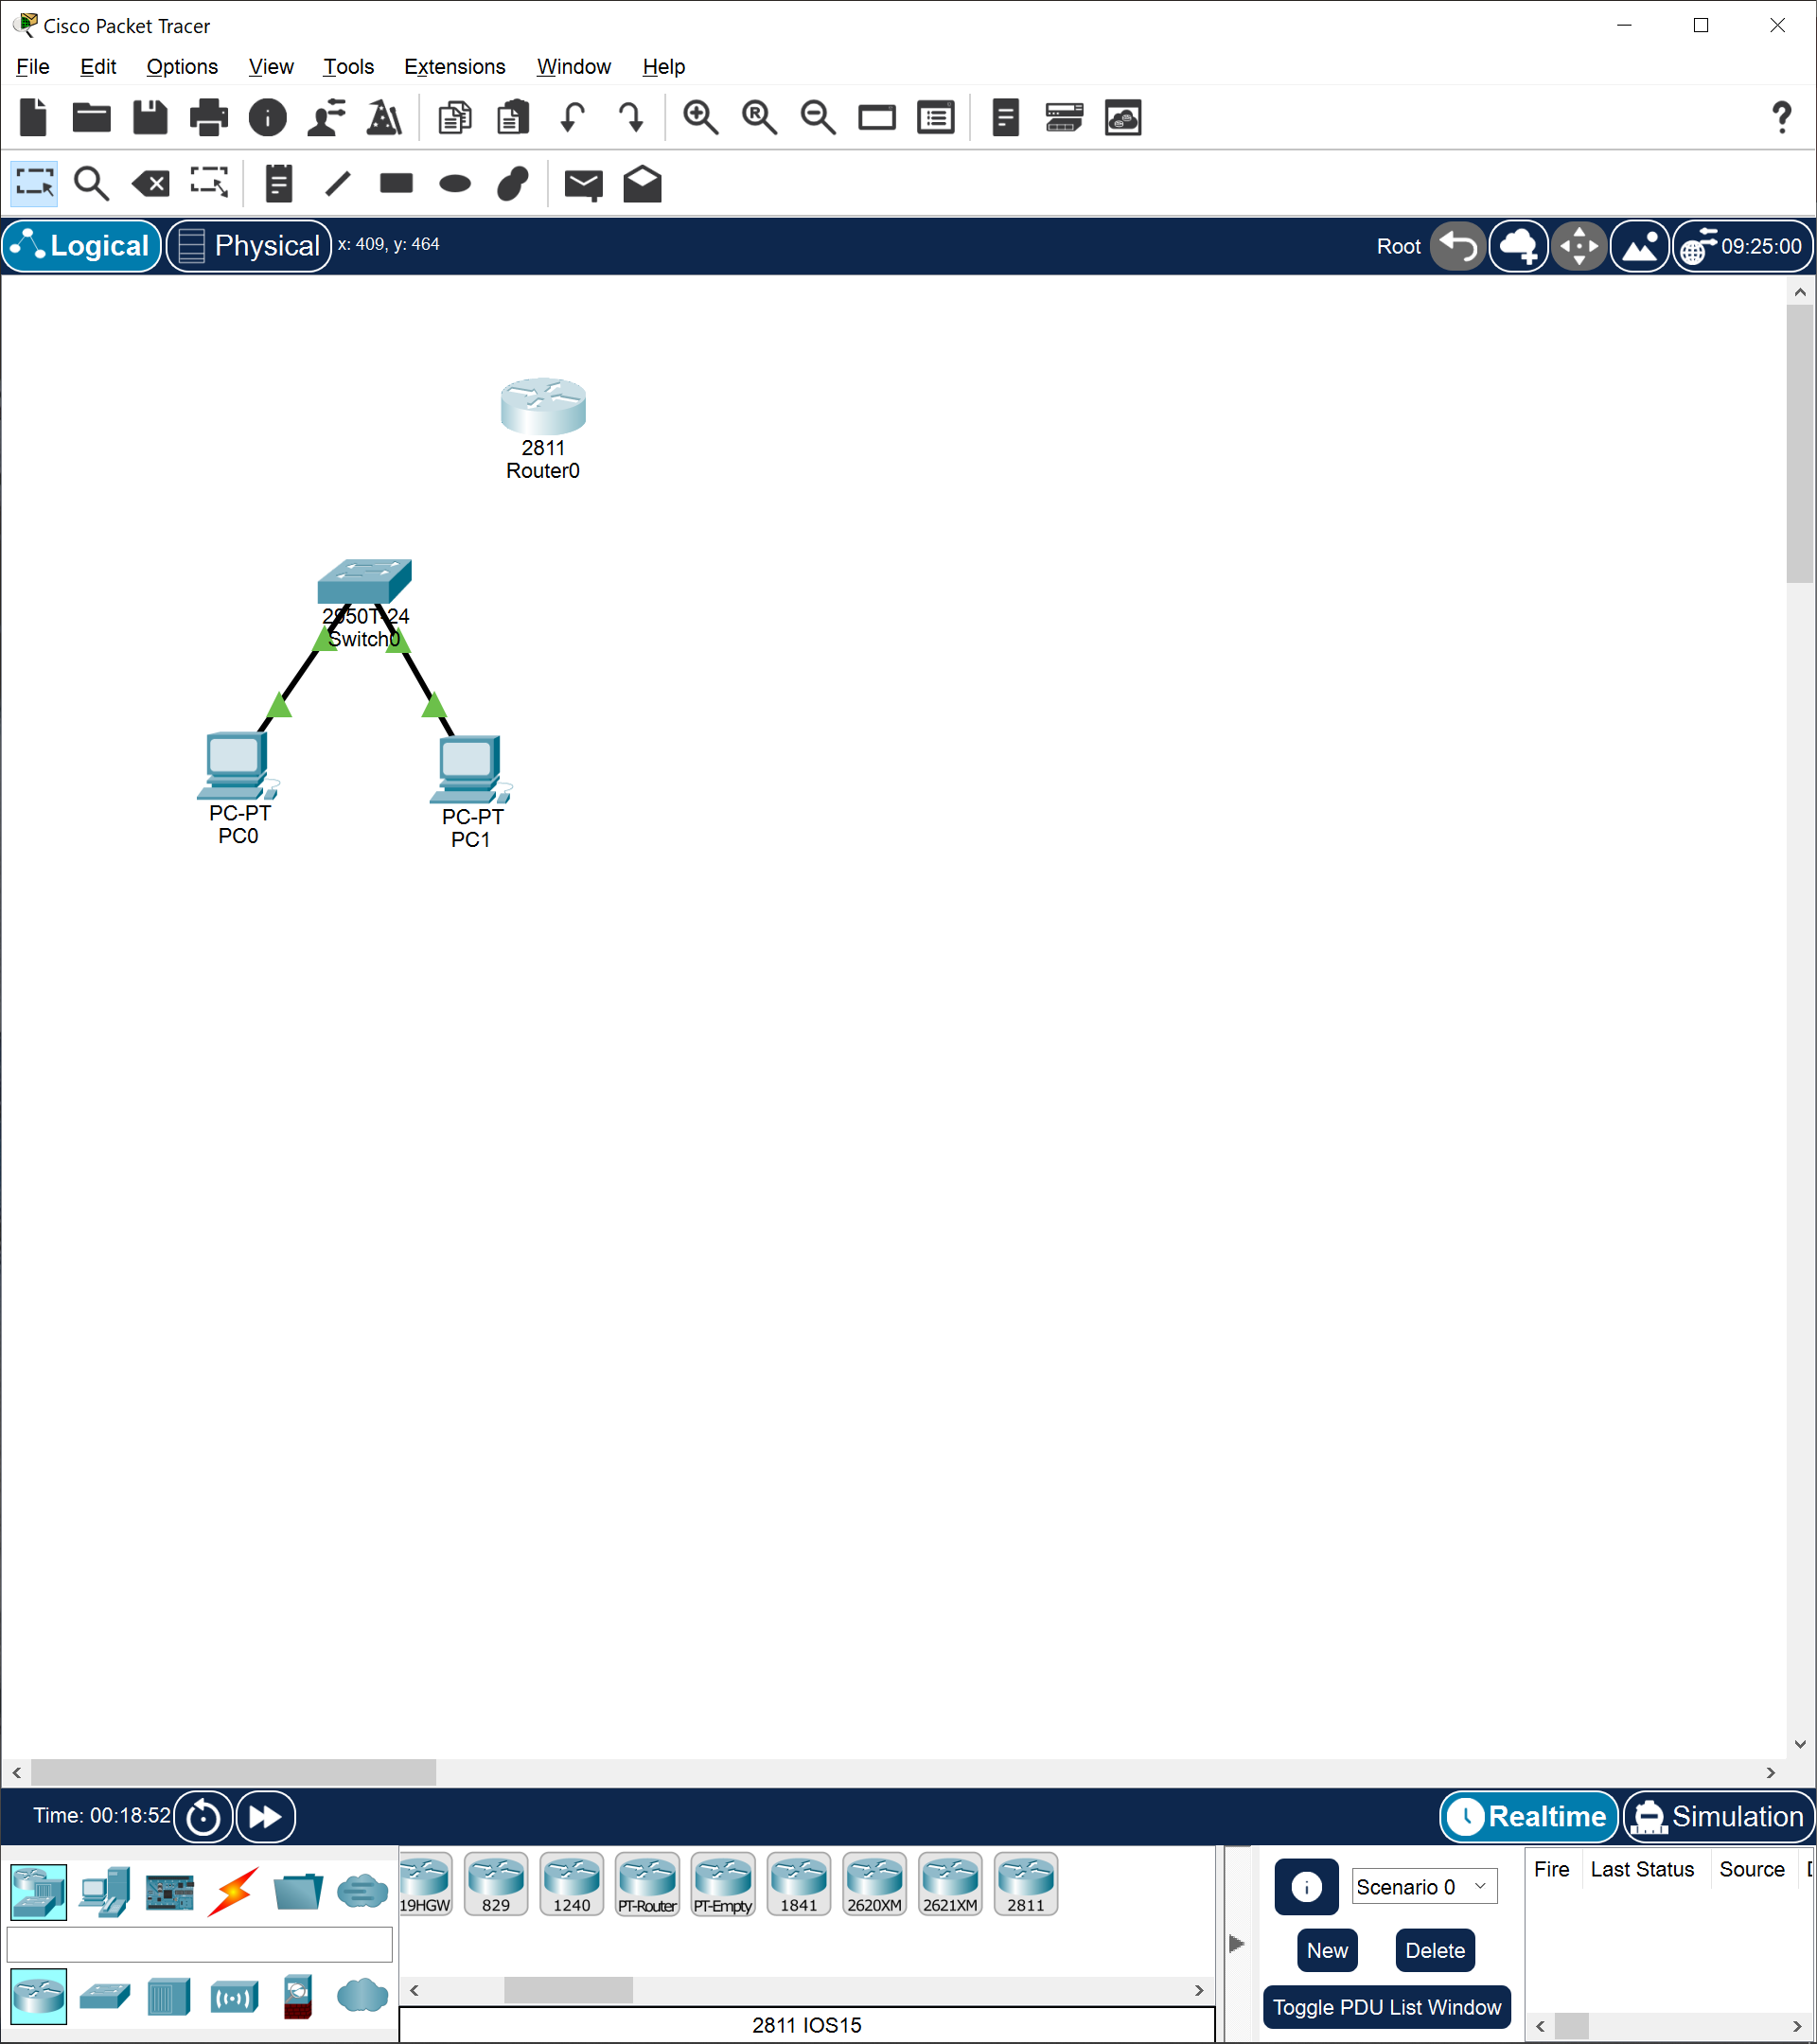
\includegraphics[width=13cm]{./step-by-step/11.PNG}
\clearpage

\noindent Let's link the router to the first computer \newline

\noindent 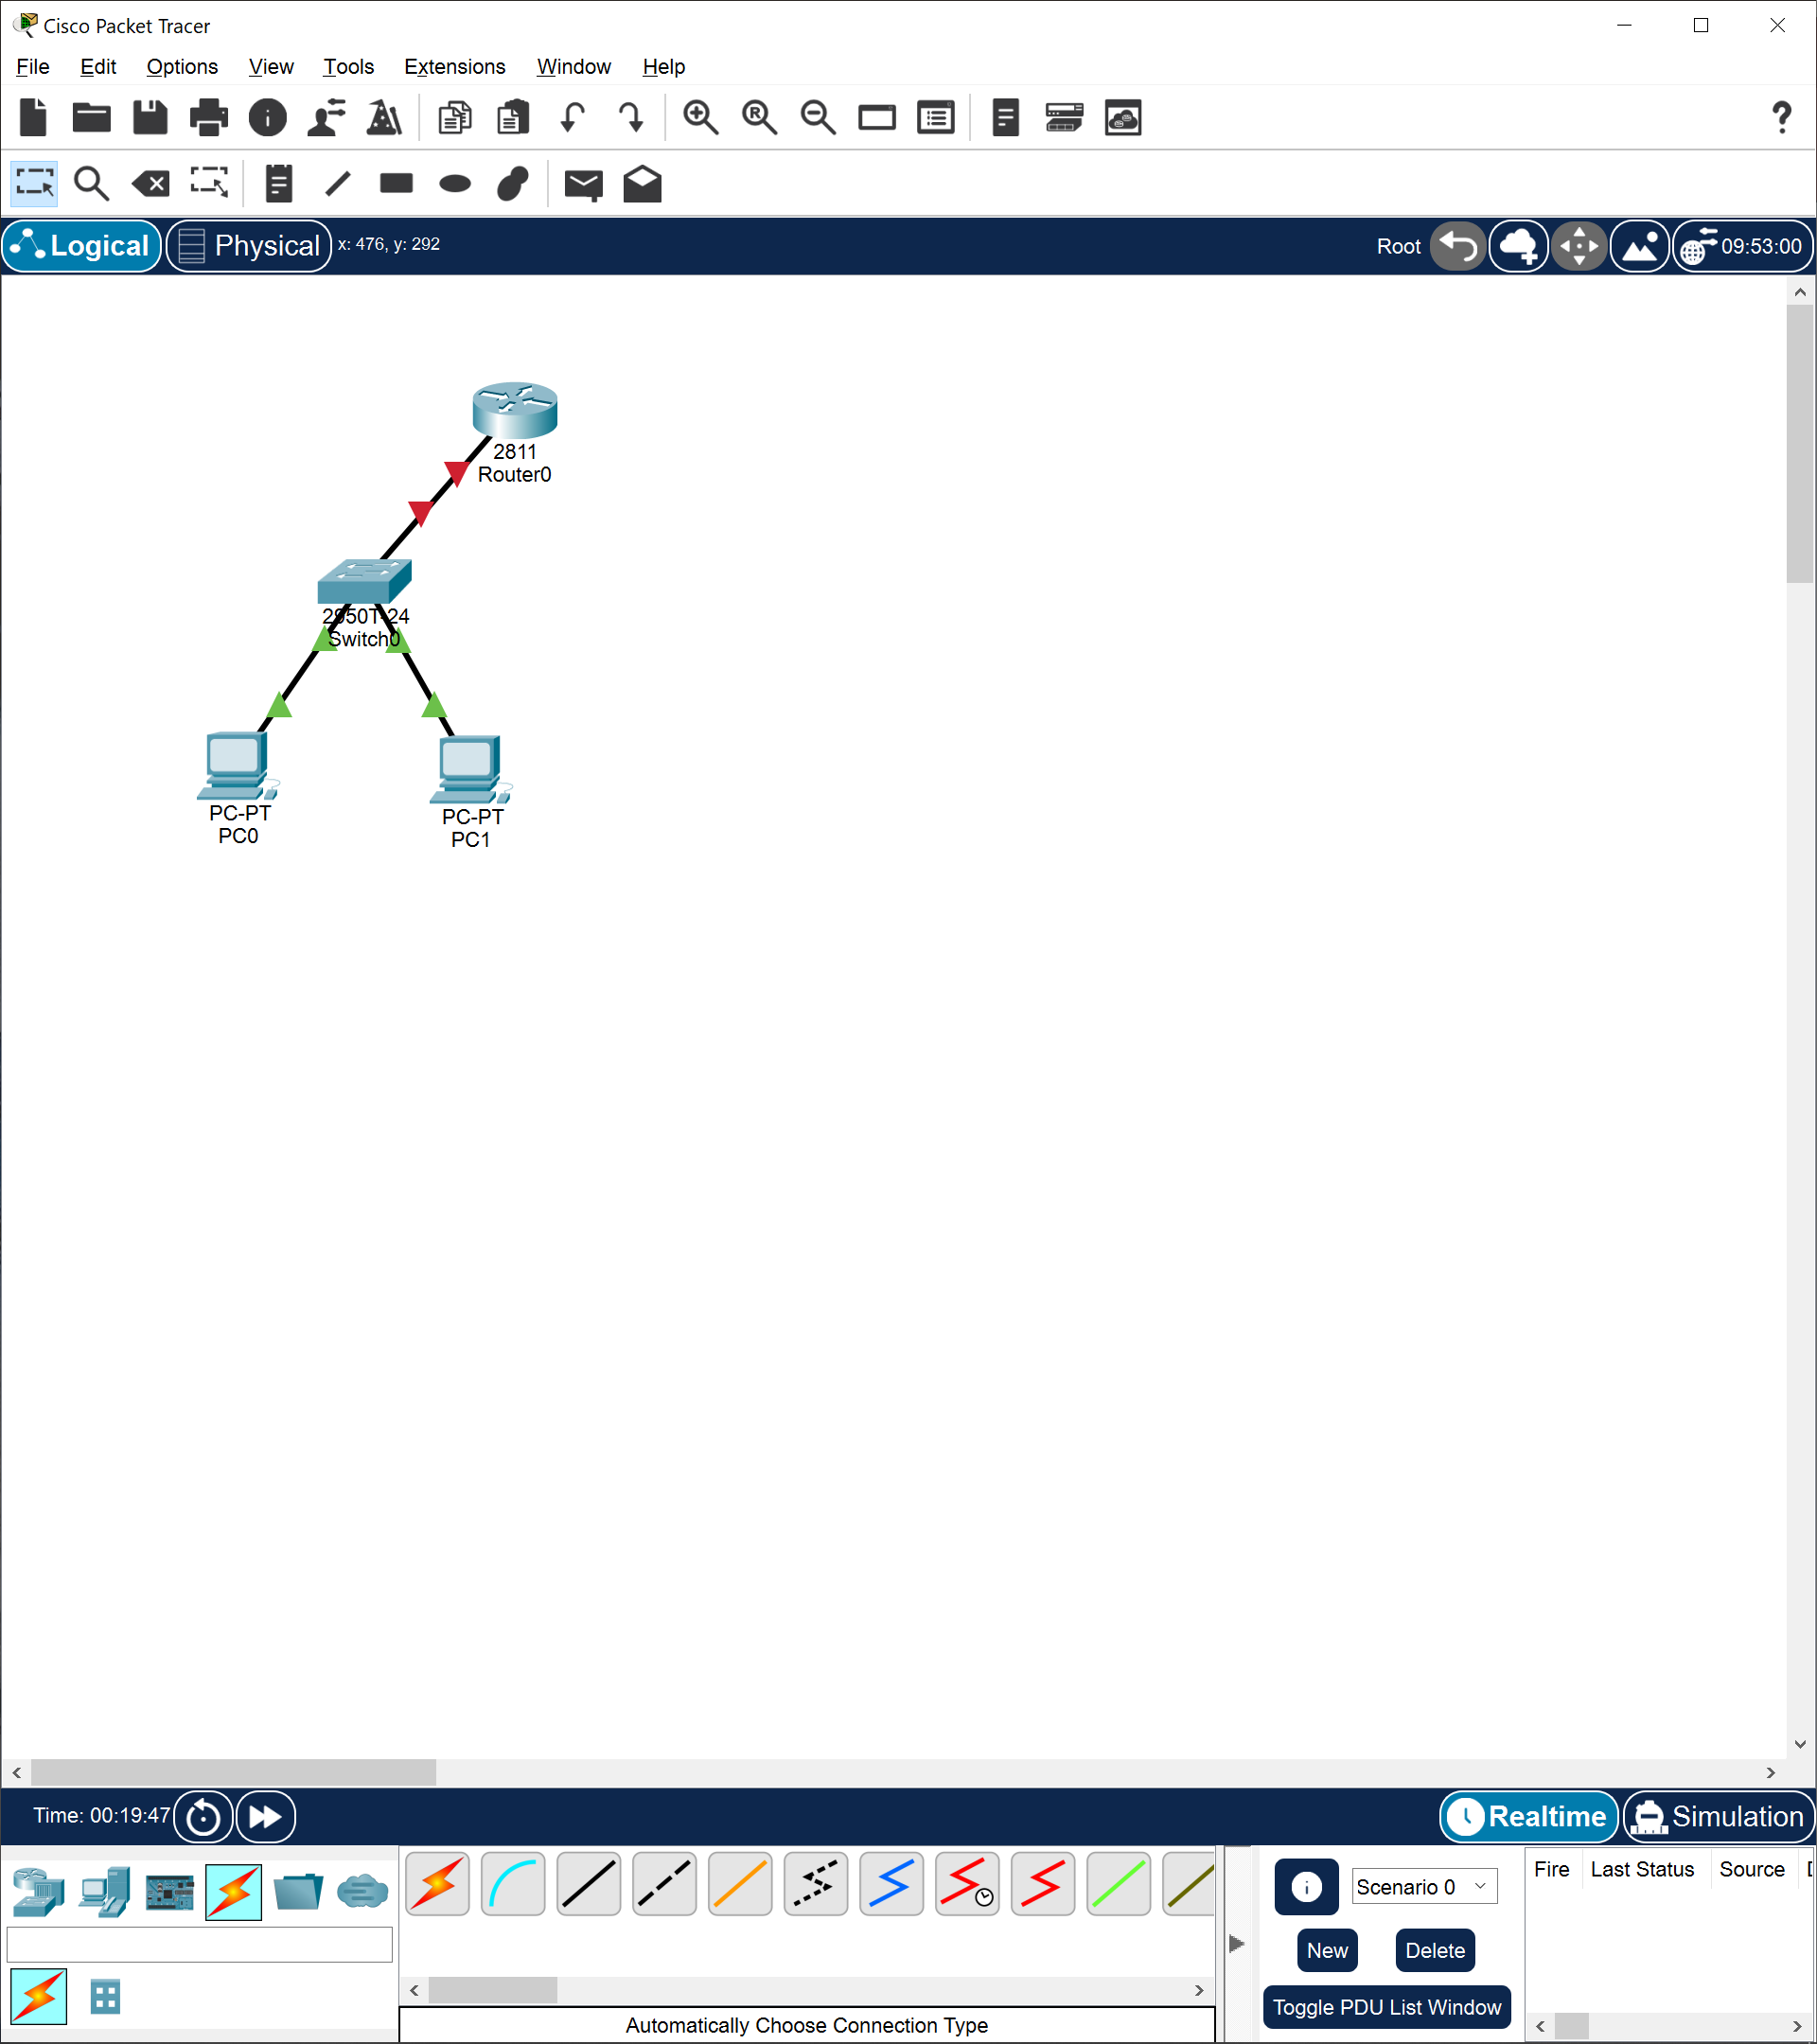
\includegraphics[width=13cm]{./step-by-step/12.PNG}
\clearpage

\noindent If you click on the router, in the config tab there is a box you need to check. That box will emulate the router being powered on \newline

\noindent 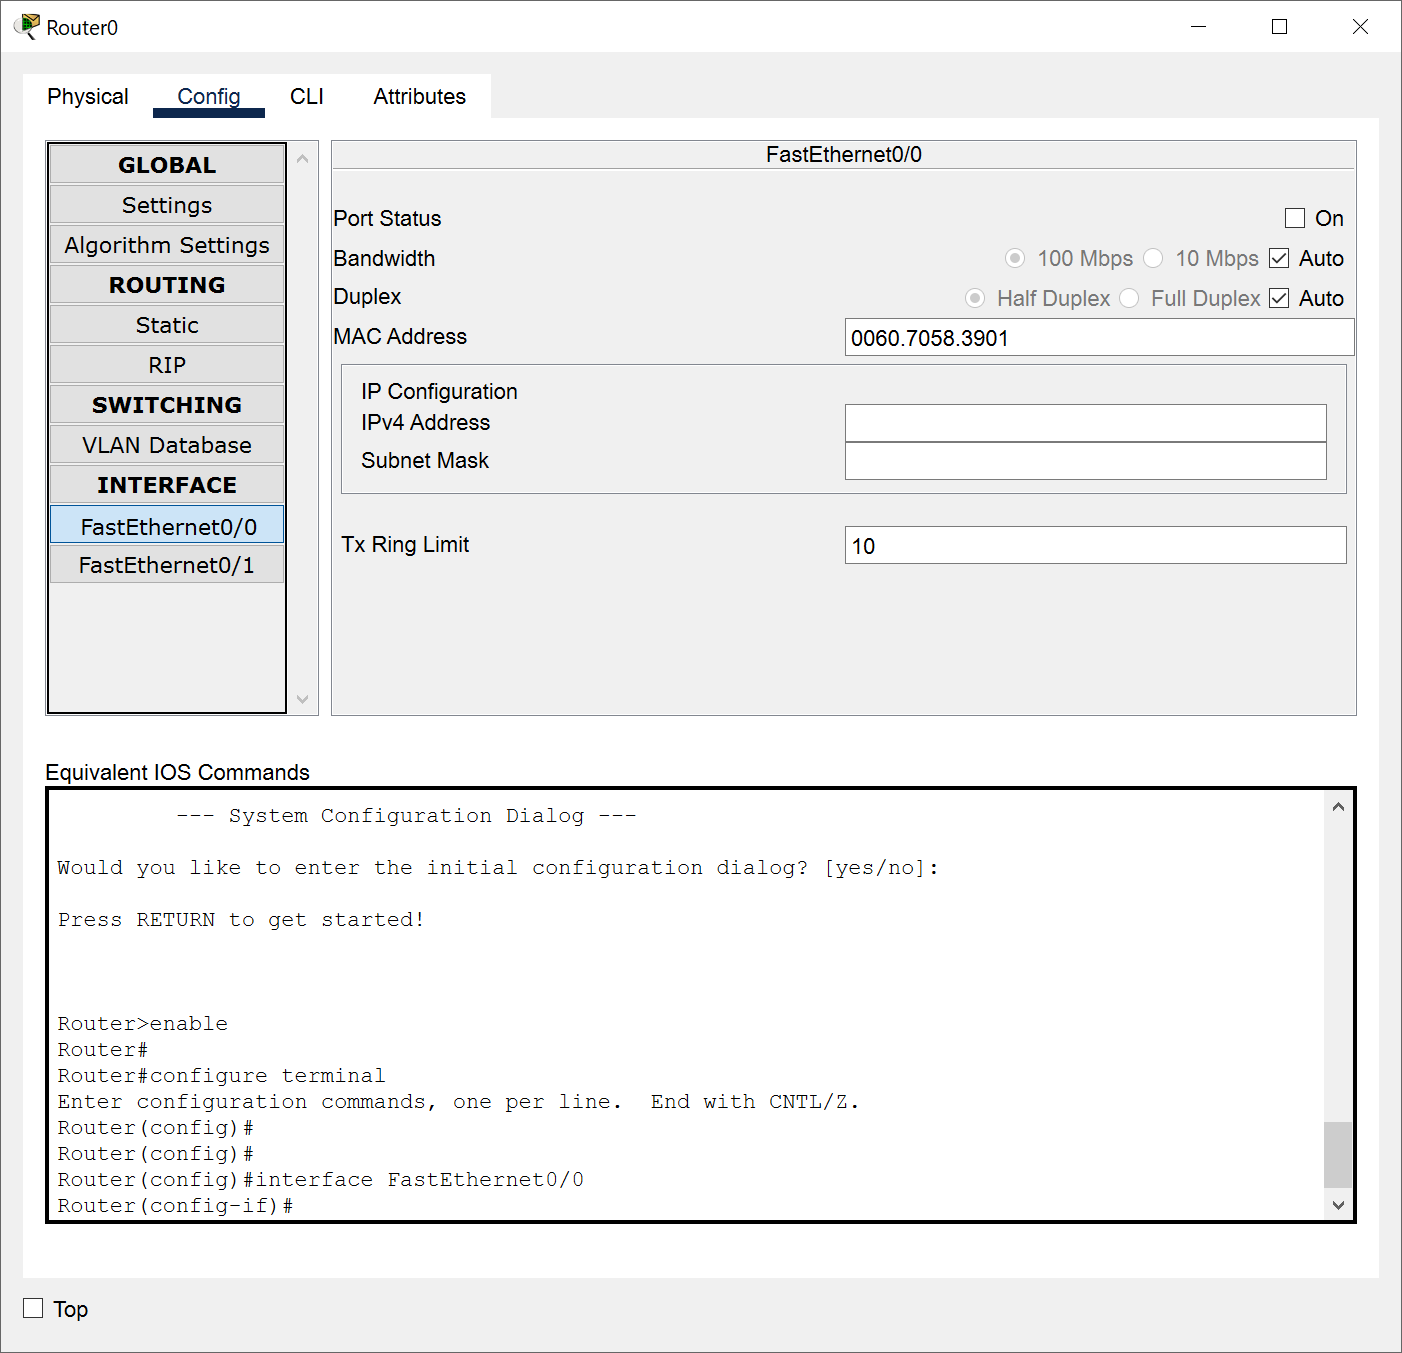
\includegraphics[width=13cm]{./step-by-step/13.PNG}
\clearpage


\noindent Once you click in the box a small tick will appear in it. This means the box is ticked and the function that box is proving is now being turned on \newline

\noindent 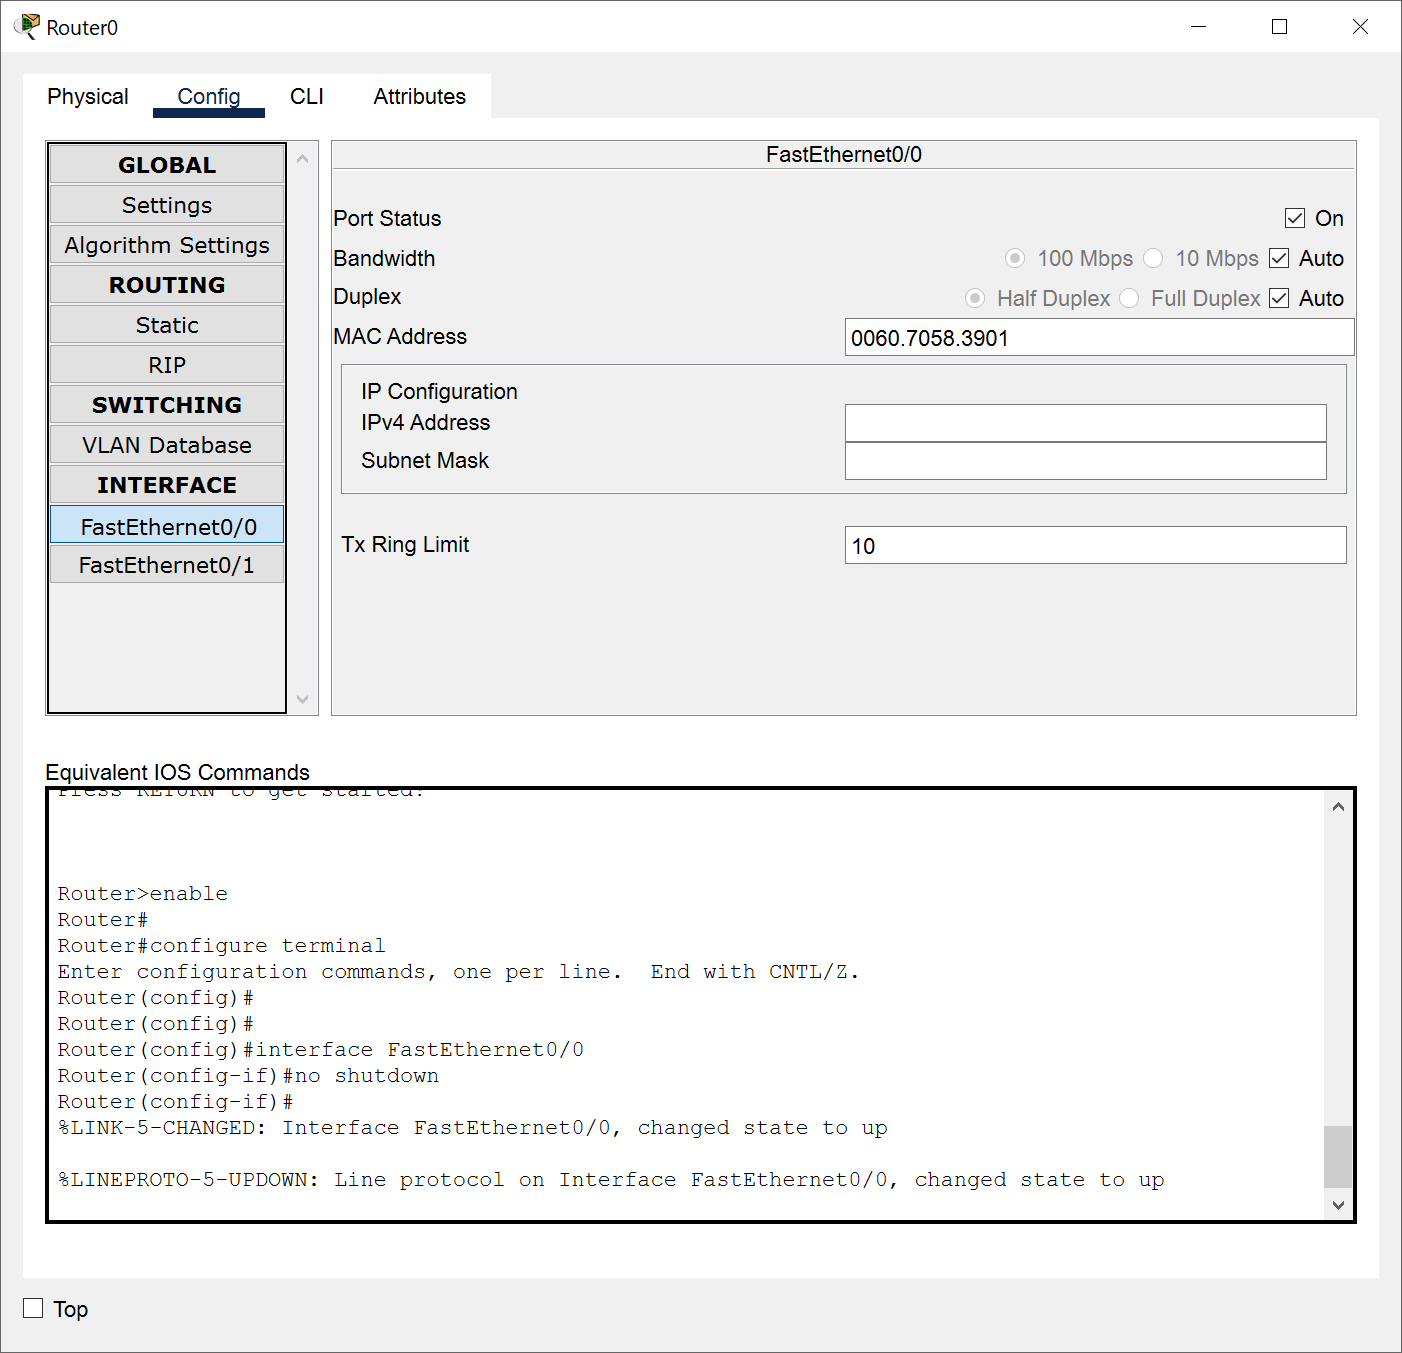
\includegraphics[width=13cm]{./step-by-step/14.PNG}
\clearpage

\noindent as a result of ticking that box now you can see the link going green wich means is enabled for data transmission \newline

\noindent 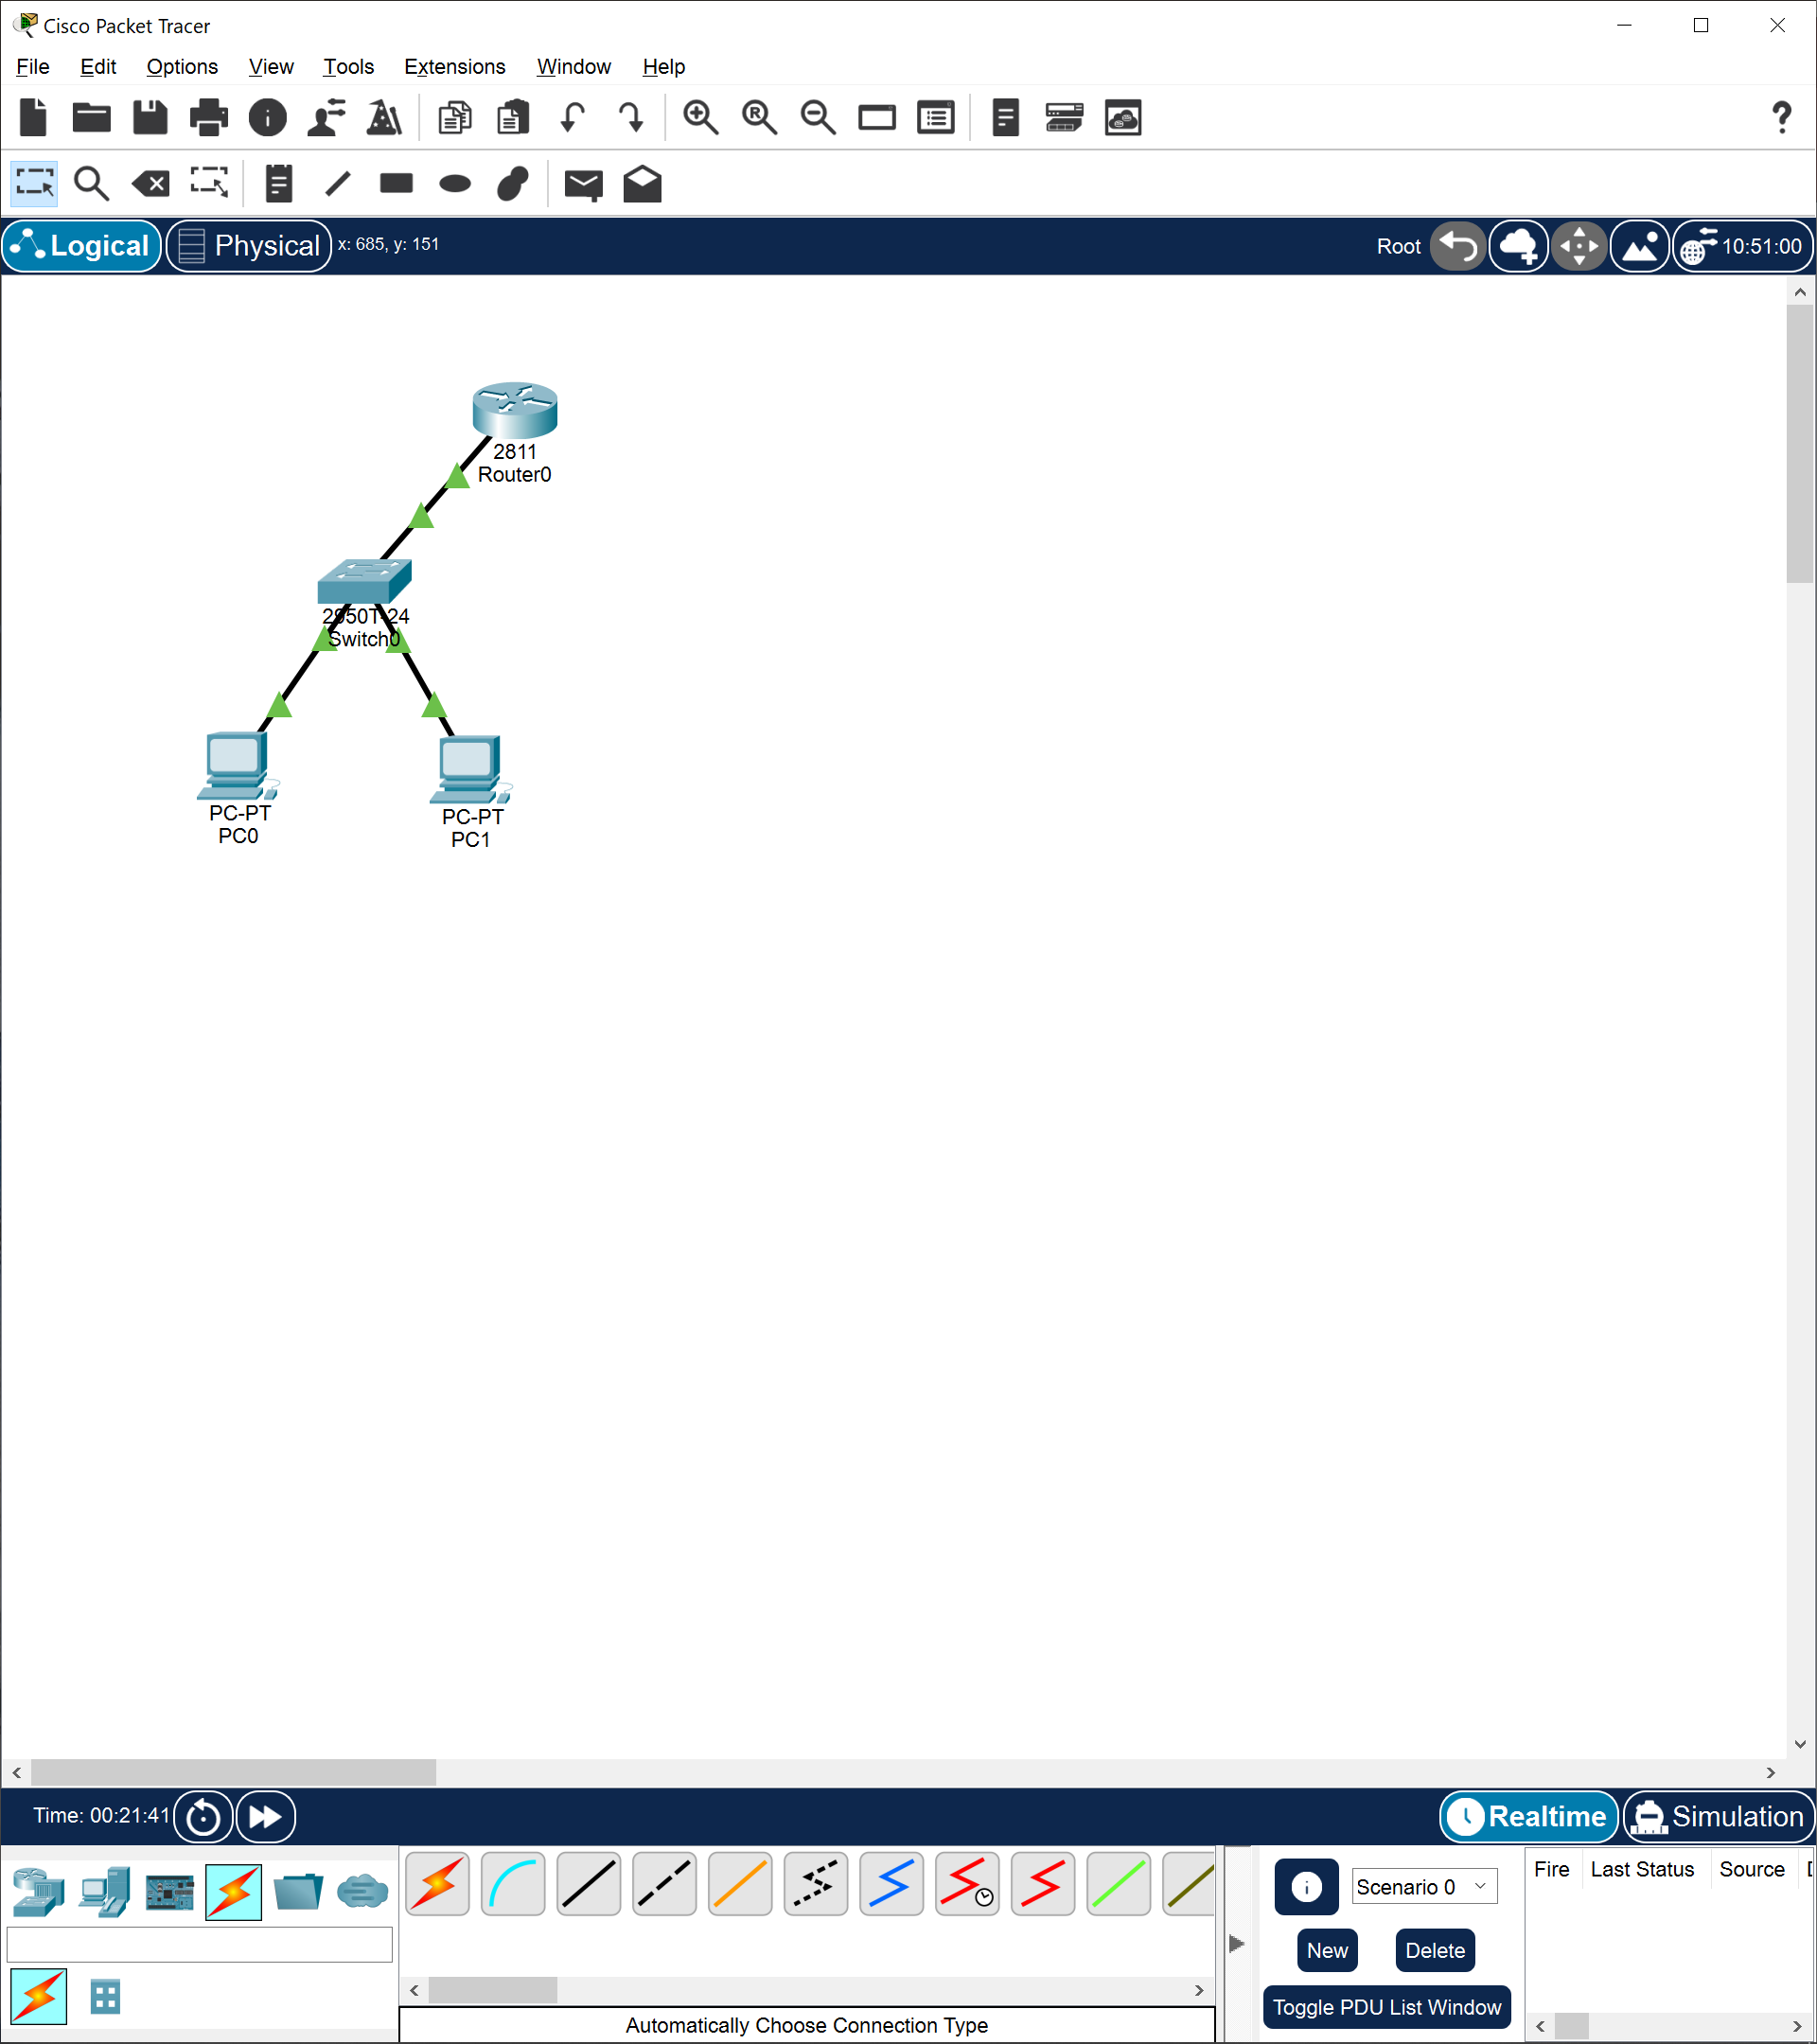
\includegraphics[width=13cm]{./step-by-step/15.PNG}
\clearpage


\noindent we only need to sort the \textbf{IP Configuration} out as well \newline

\noindent 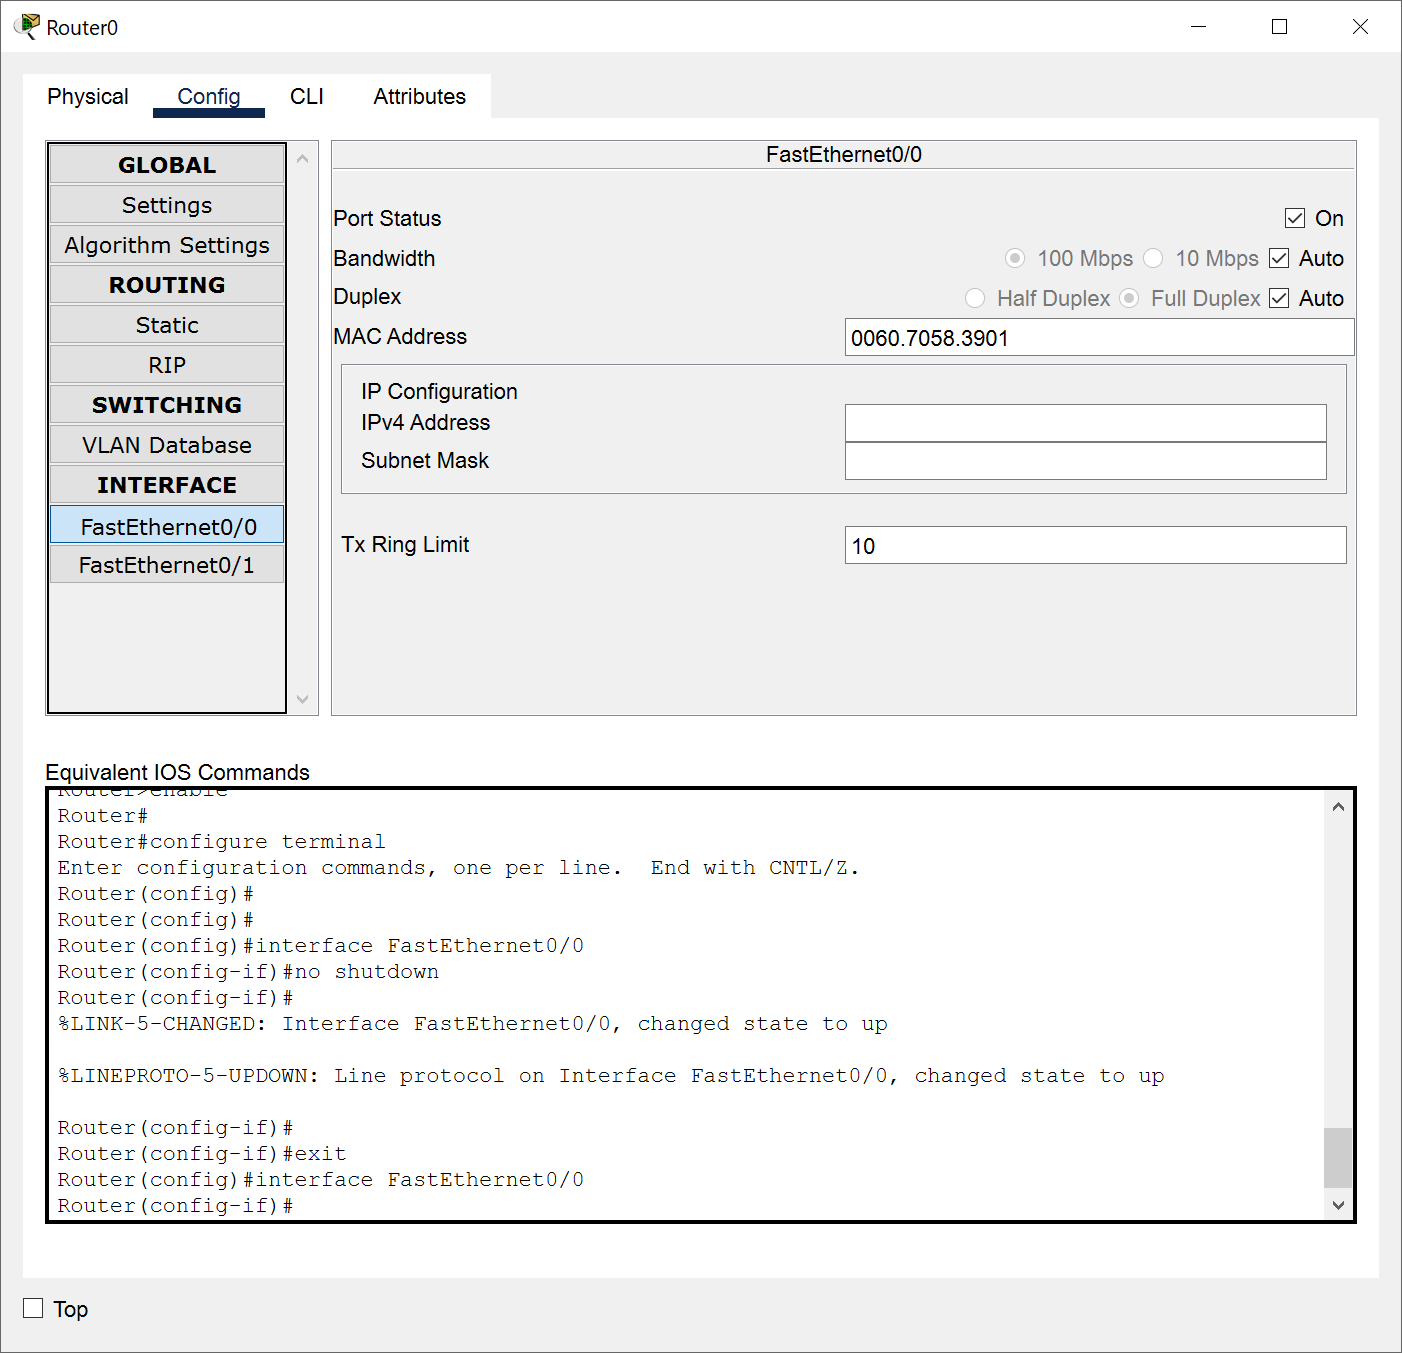
\includegraphics[width=13cm]{./step-by-step/16.PNG}
\clearpage


\noindent Now, because the subnet mask indicates how many values can you actually use this means we can use

\[ 255 values - X values \]

\noindent where \emph{X} is the number in a subnetmask like \emph{Z.Y.W.X} which in the case of \emph{255.255.255.0} will be

\[ 255 - 0\]

\noindent which returns 255 values but because we start counting from 0 we can go up to 254.
In the following example you can see the value 0 being accepted as a valid value \newline 

\noindent 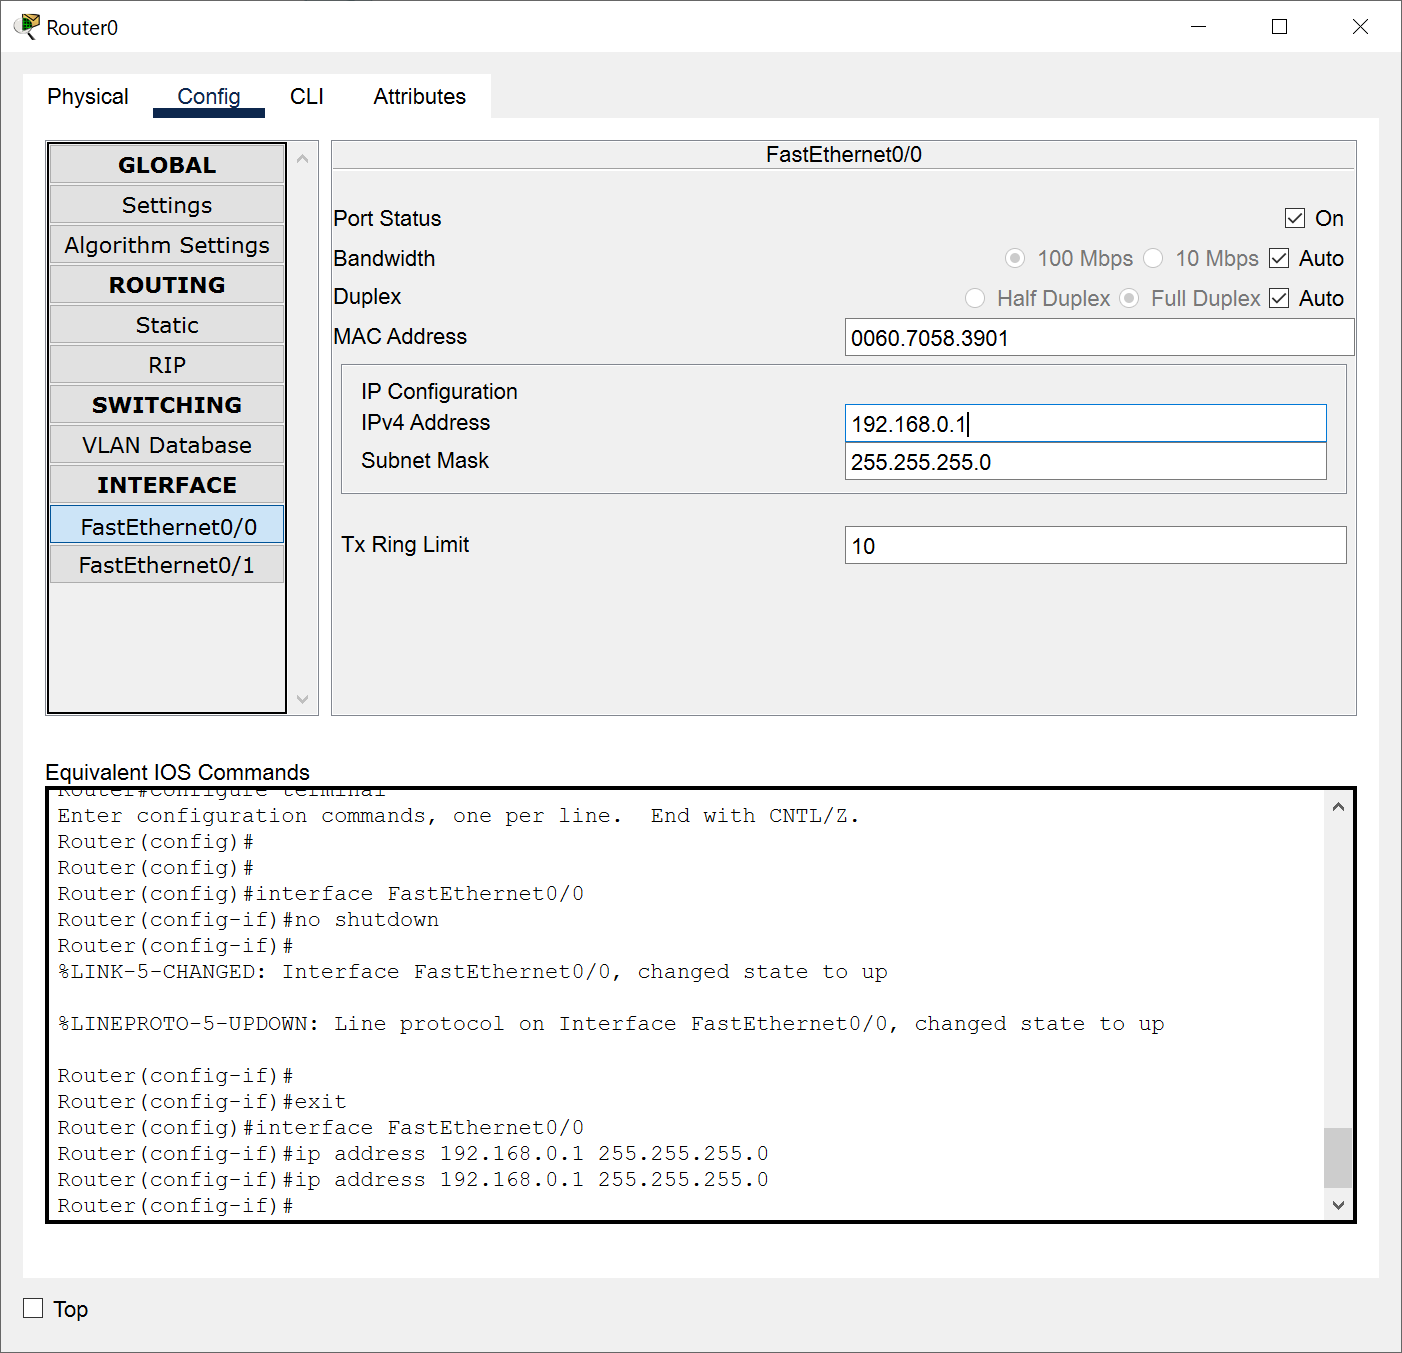
\includegraphics[width=13cm]{./step-by-step/17.PNG}
\clearpage


\noindent Let's pick up PC1 console and ping all devices in the 192.168.0.1 network. The ping works \newline

\noindent 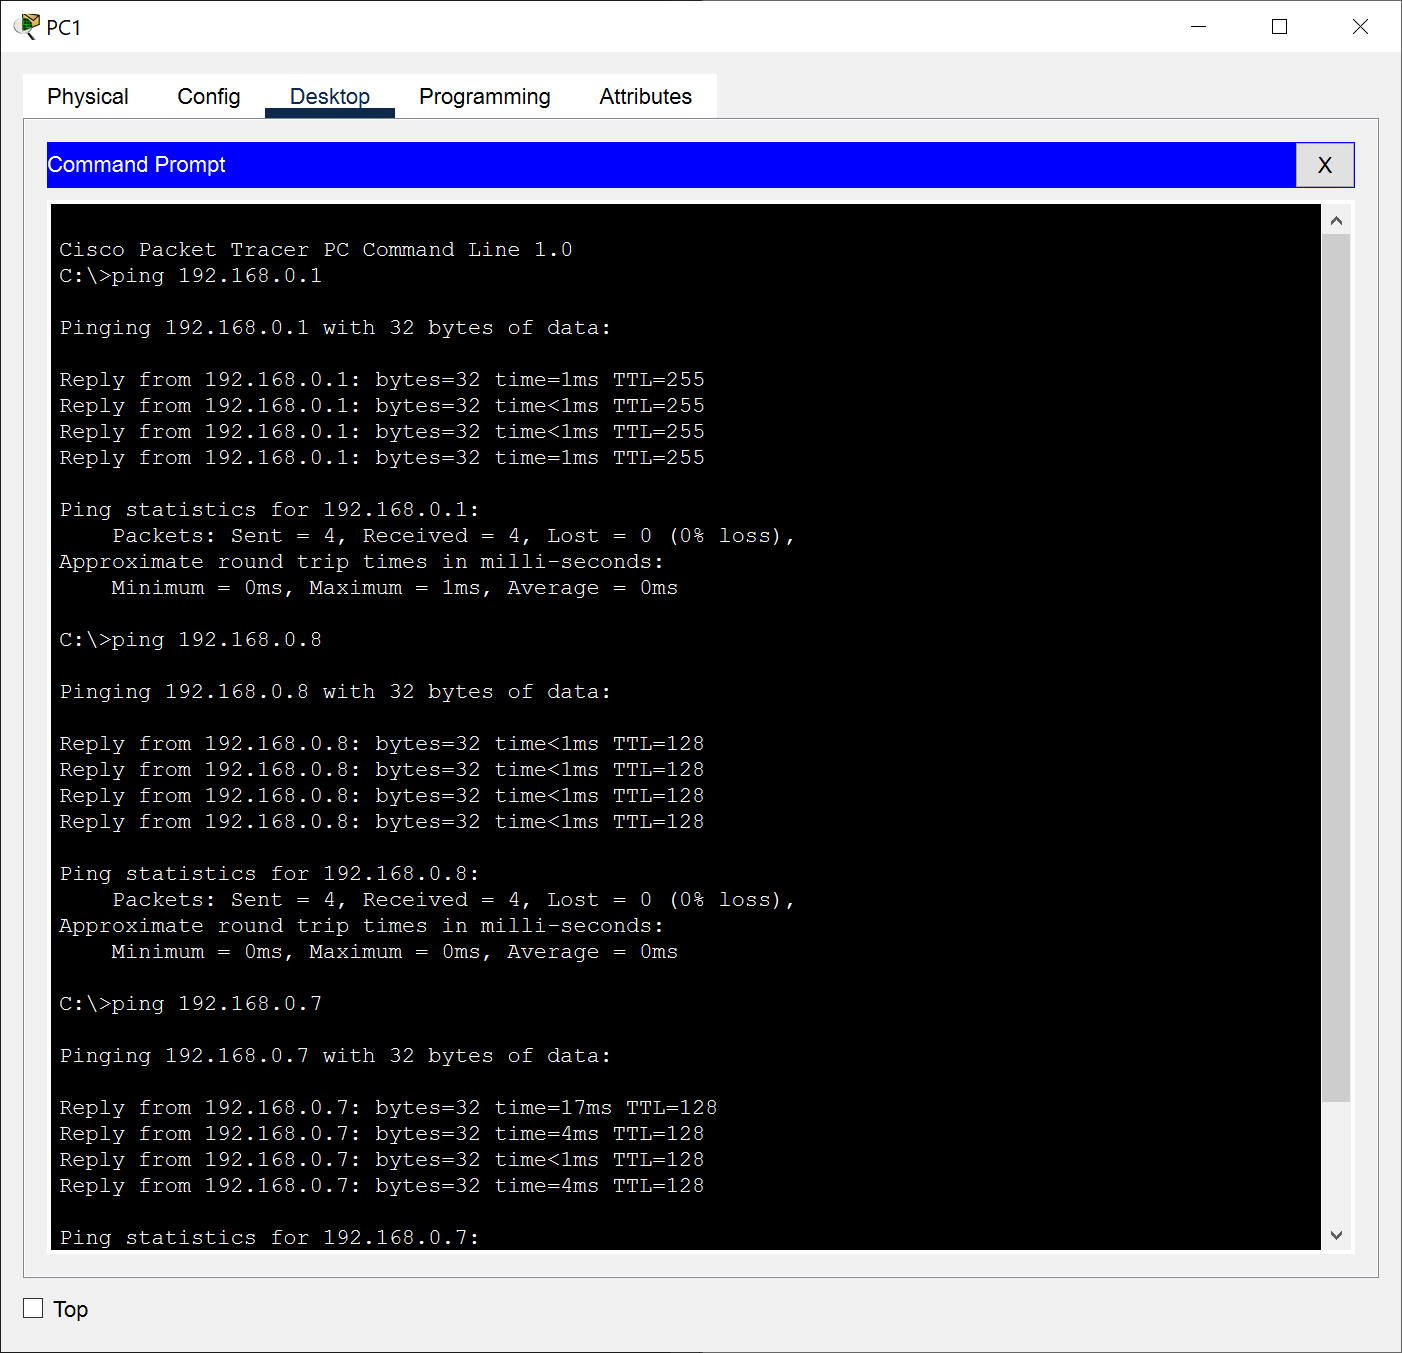
\includegraphics[width=13cm]{./step-by-step/18.PNG}
\clearpage

\noindent Let's create a copy of the subnetwork we have already. The gateway will be this time 
\[192.168.1.1\] \newline
 
\noindent 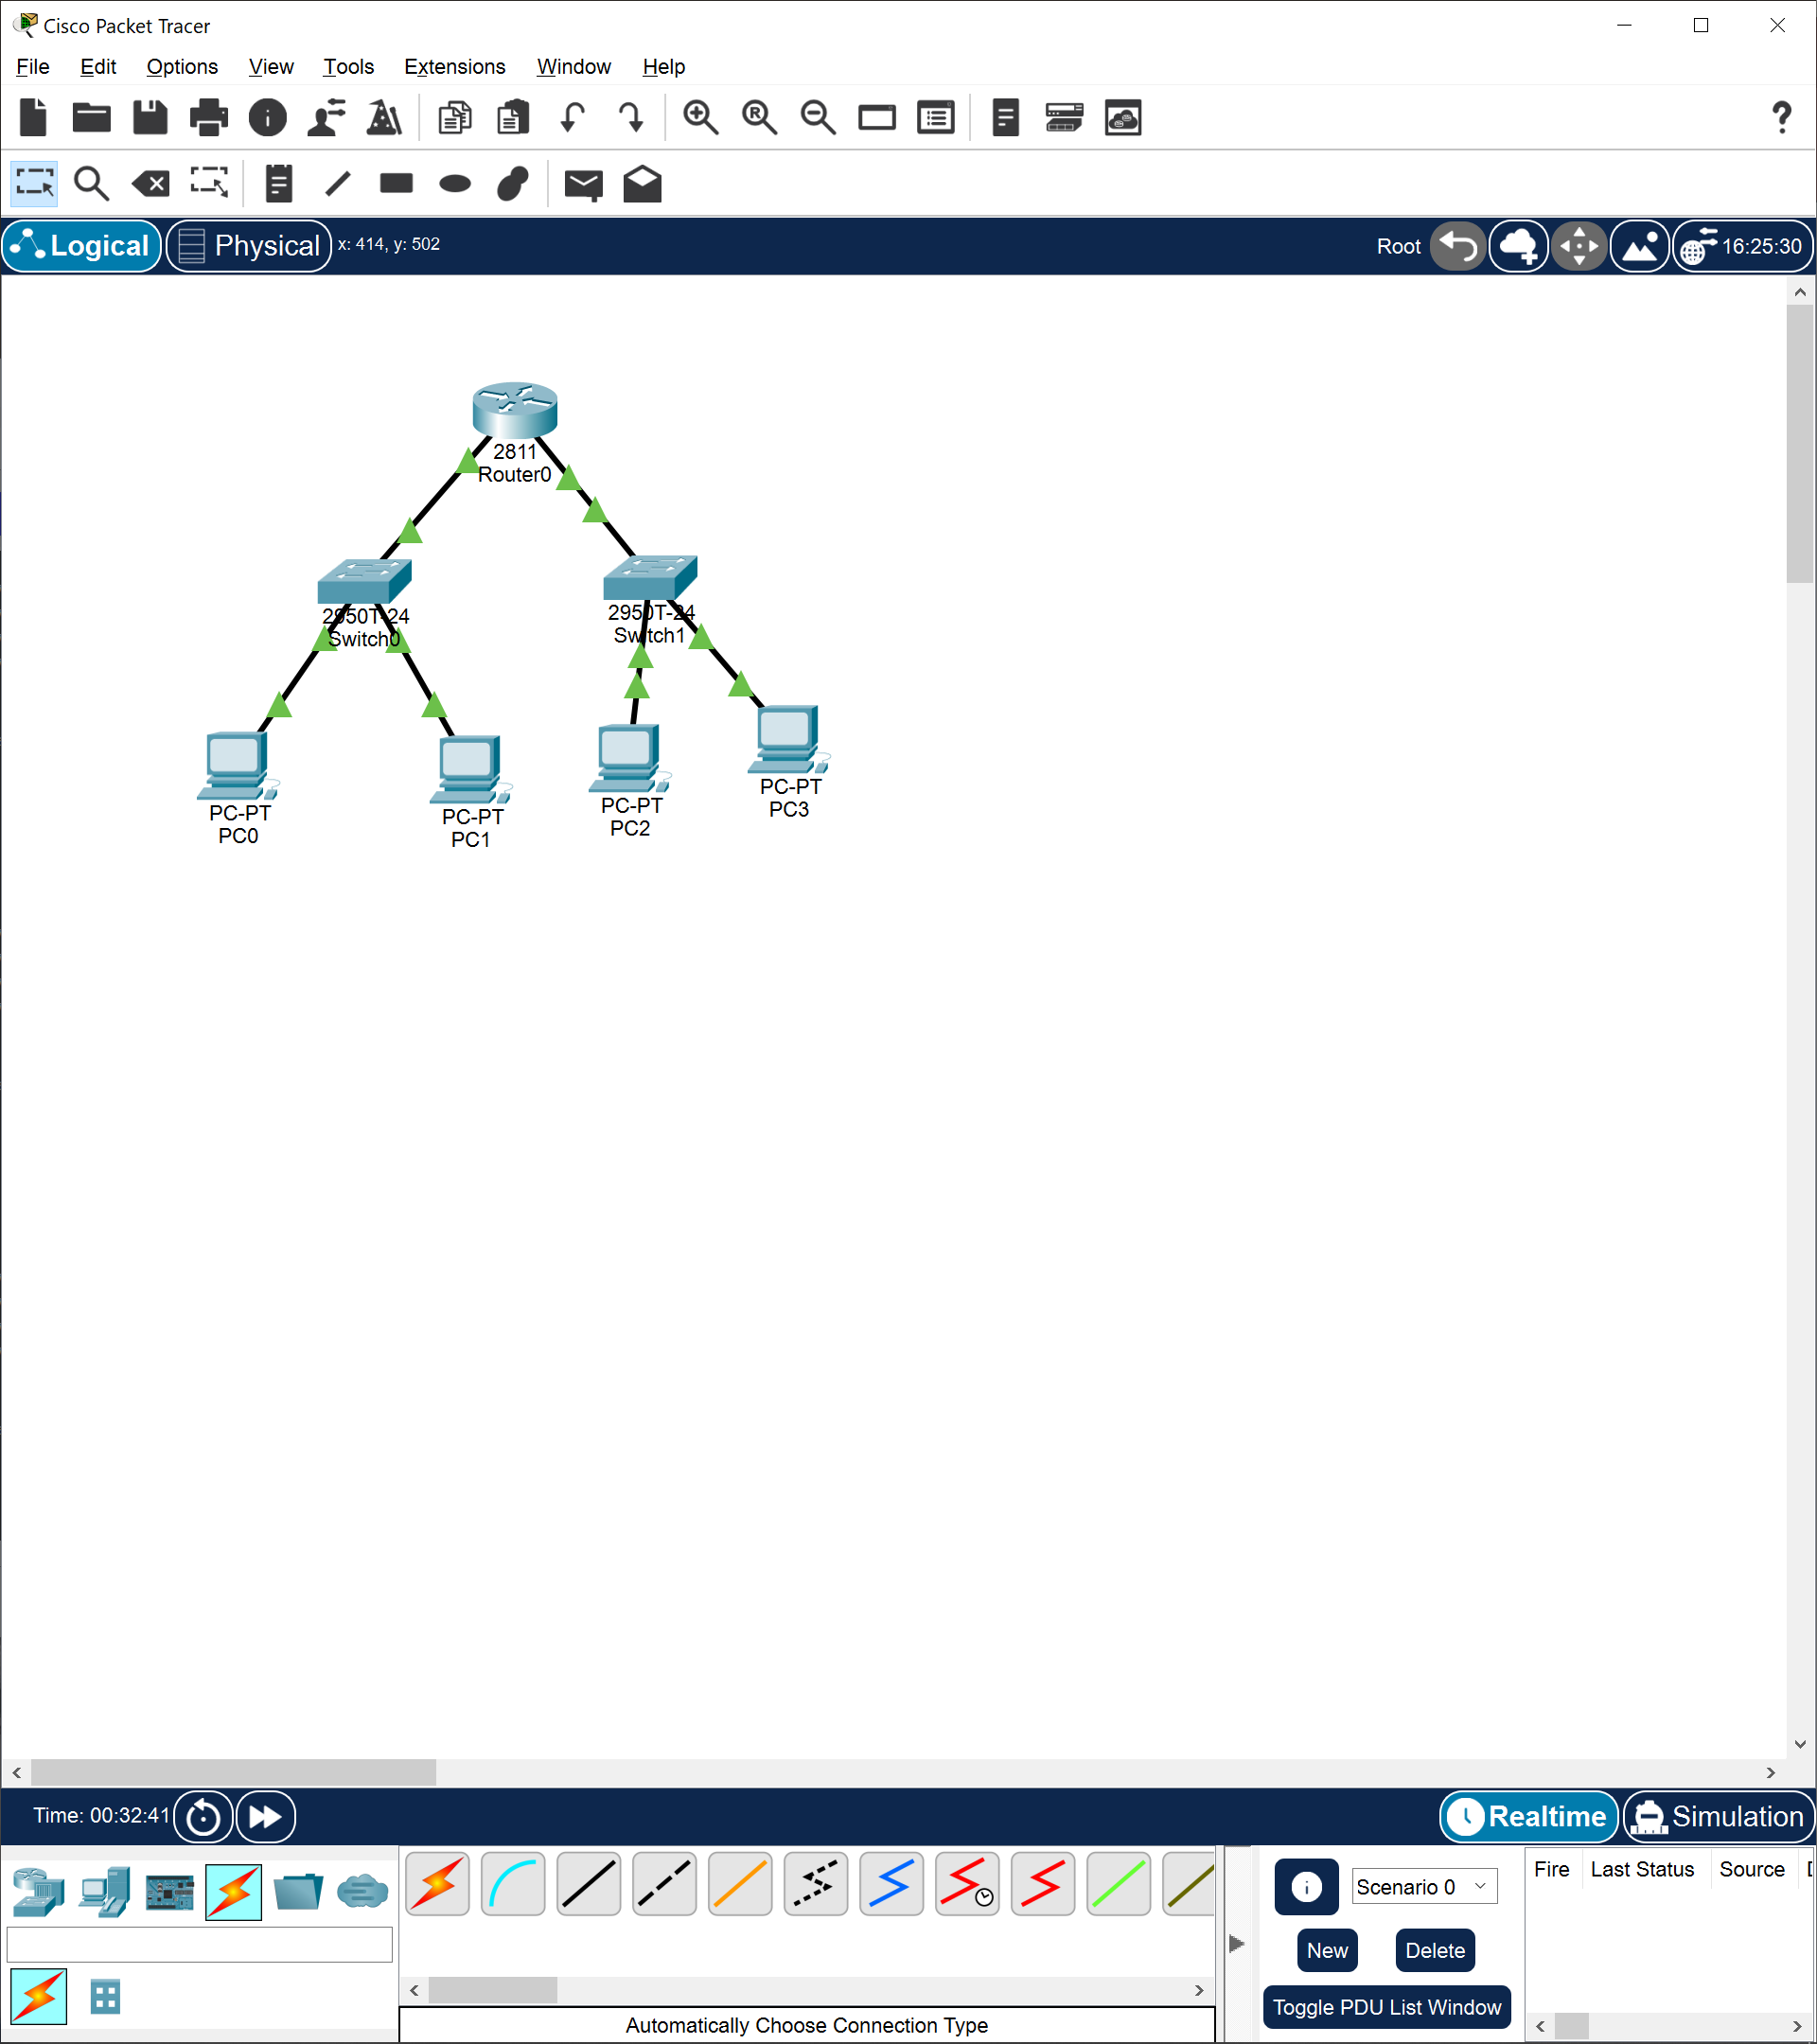
\includegraphics[width=13cm]{./step-by-step/19.PNG}
\clearpage

\subsubsection{expanding the network}
\noindent Let's add a printer with the following IP
\[192.168.1.20\] \newline

\noindent 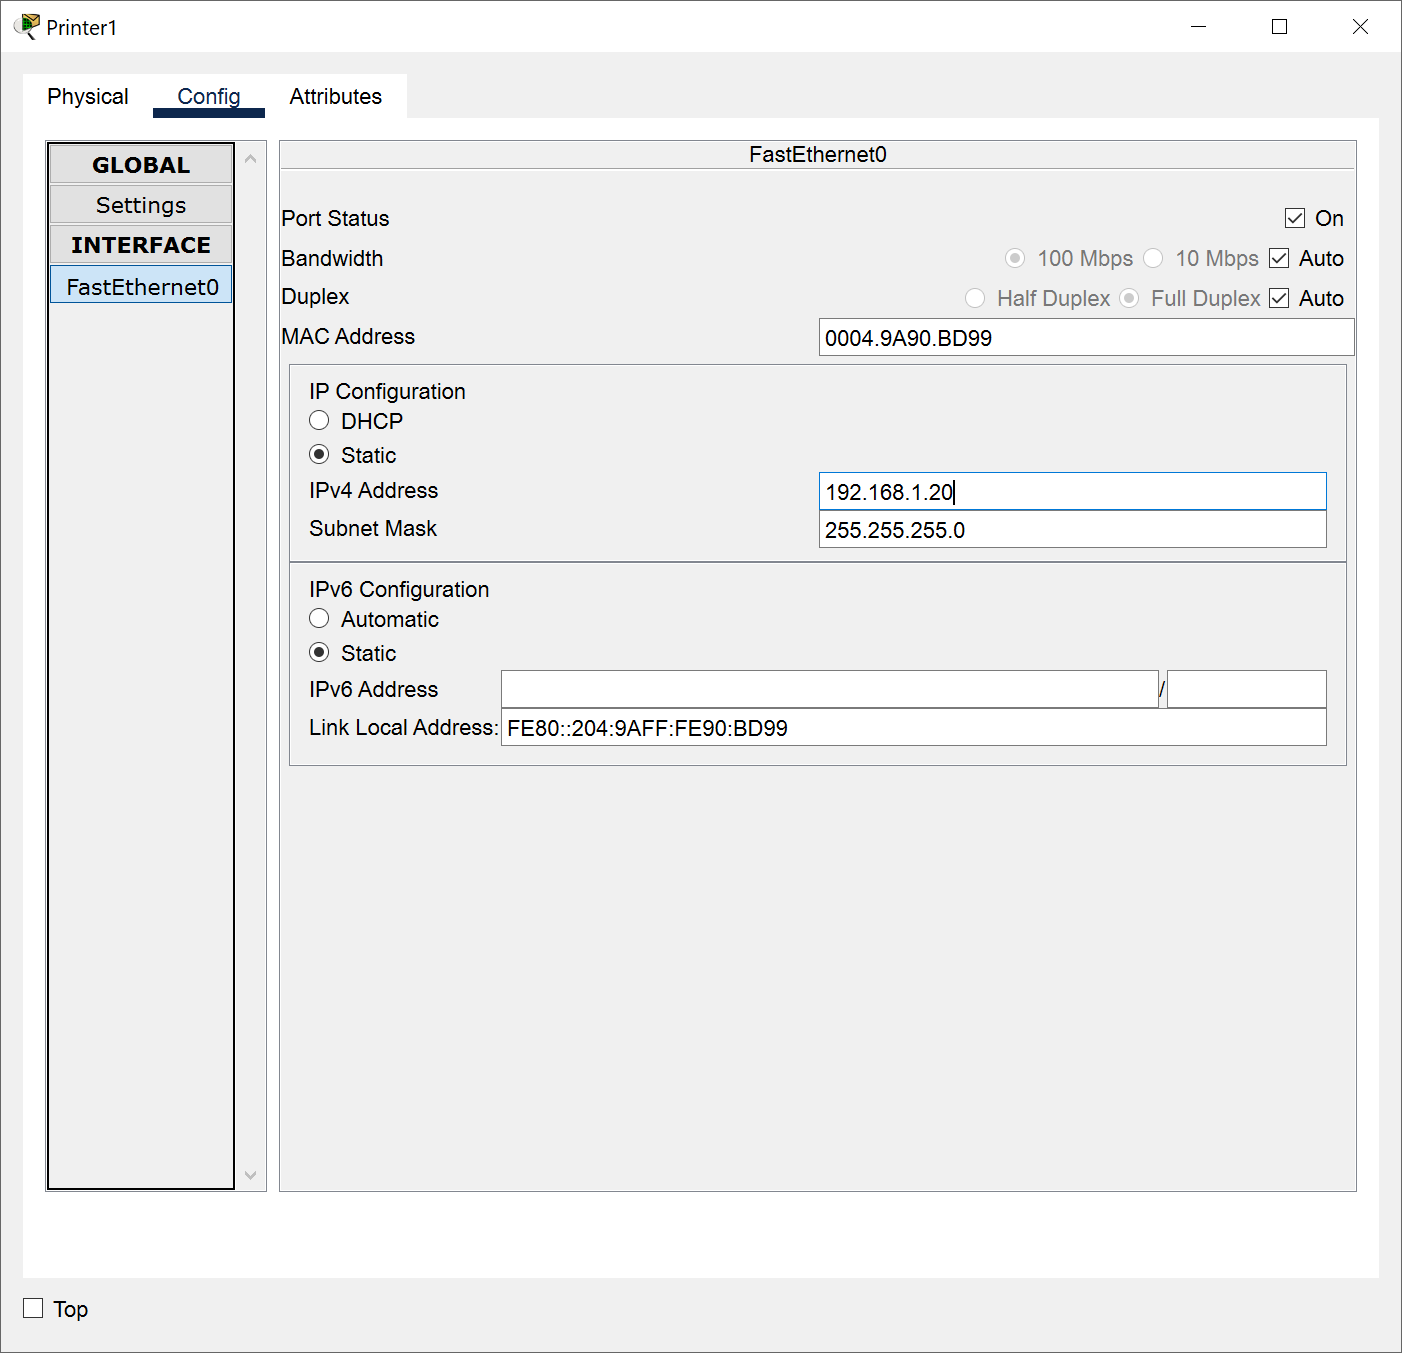
\includegraphics[width=13cm]{./step-by-step/20.PNG}
\clearpage

\noindent Let's ping the printer from PC0\newline

\noindent 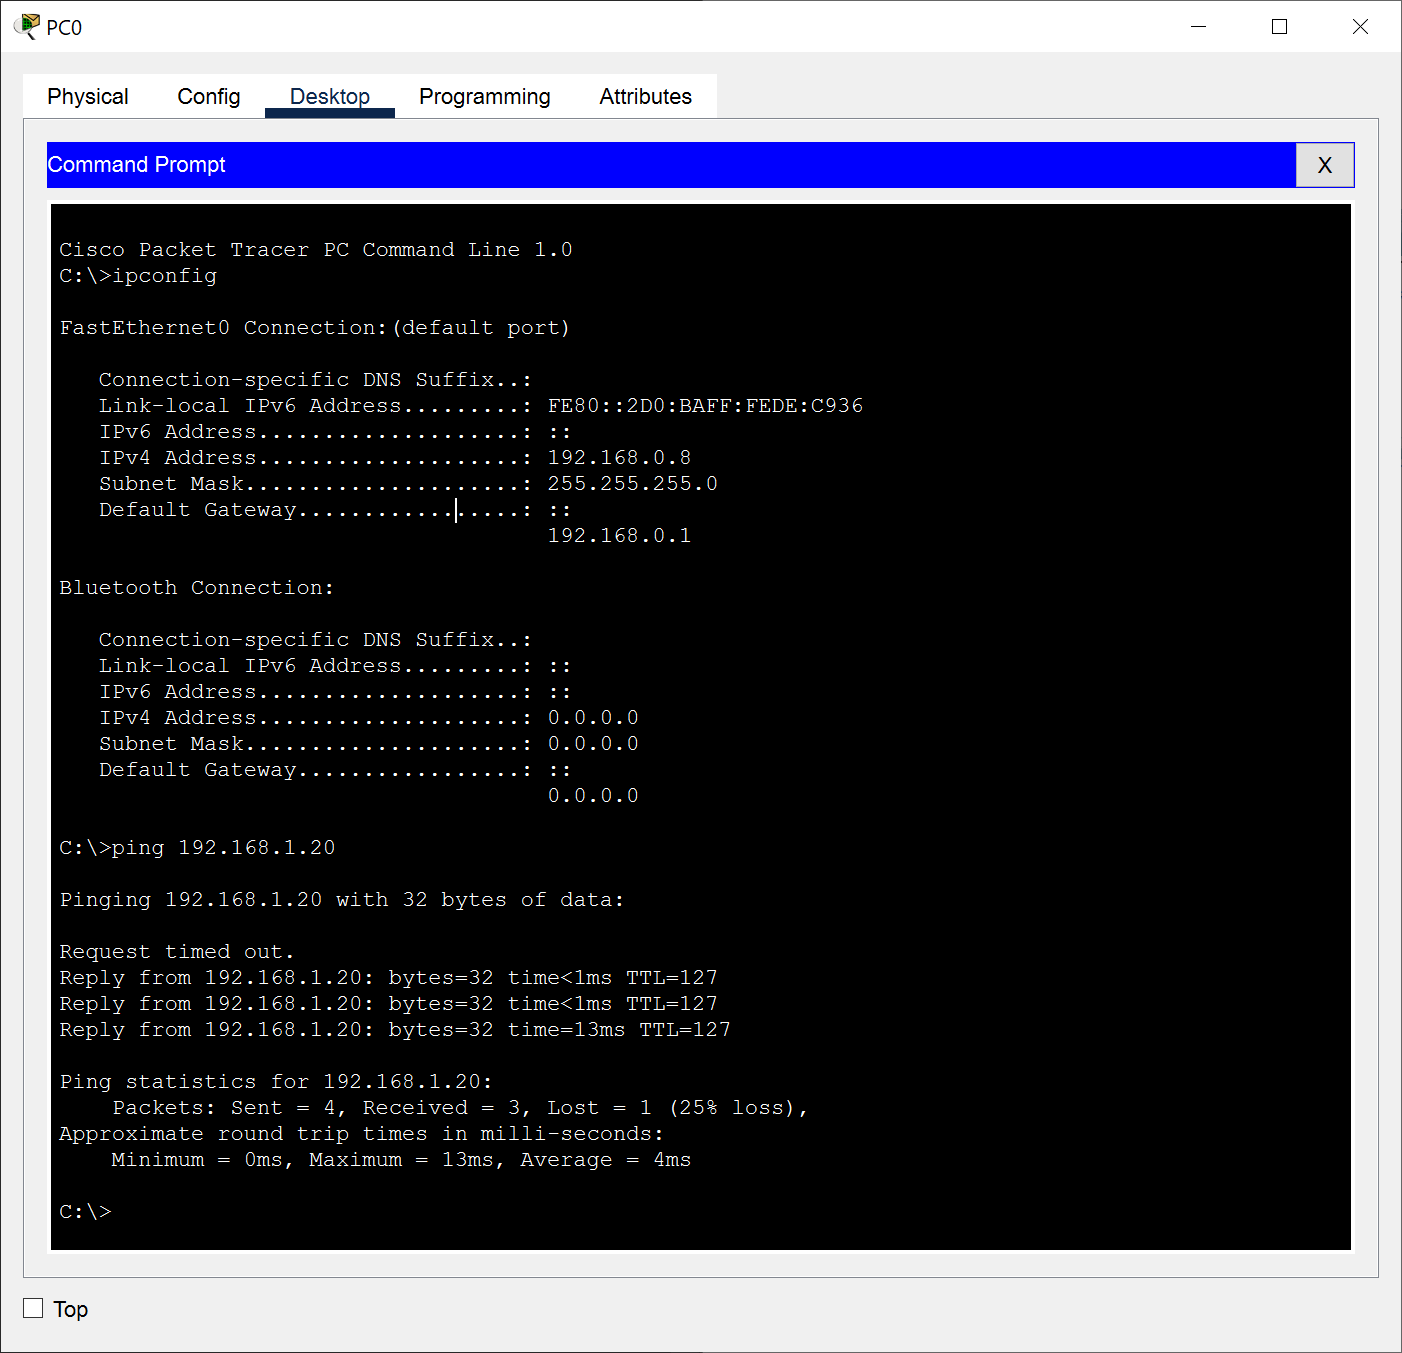
\includegraphics[width=13cm]{./step-by-step/21.PNG} \newline
\noindent We can safely assume the network is working
\clearpage

\section{Power over Ethernet}
Power over Ethernet is a technique for delivering DC power to devices over copper Ethernet cabling, eliminating the need for separate power supplies and outlets. While PoE doesn't add Ethernet data capabilities, it does offer expanded options for how and where Ethernet end devices can be placed.

%\section{LAN status LEDs}

\section{Topology}

It's a layout of physical devices. It's an arrangement of devices

\subsection{Star Topology}

In star topology, every peripheral node (computer workstation or any other peripheral) is connected to a central node called a hub or switch. The hub is the server and the peripherals are the clients. The network does not necessarily have to resemble a star to be classified as a star network, but all of the peripheral nodes on the network must be connected to one central hub. All traffic that traverses the network passes through the central hub, which acts as a signal repeater.

\subsubsection{PROs}

\begin{itemize}
\item {simplicity of adding additional nodes}
\item {is the easiest topology to design and implement}
\end{itemize}

\subsubsection{CONs}

\begin{itemize}
\item {the hub represents a single point of failure}
\item {Since all peripheral communication must flow through the central hub, the aggregate central bandwidth forms a network bottleneck for large clusters}
\end{itemize}

\clearpage

\subsection{Ring Topology}

A ring topology is a daisy chain in a closed loop. Data travels around the ring in one direction. When one node sends data to another, the data passes through each intermediate node on the ring until it reaches its destination. The intermediate nodes repeat (re transmit) the data to keep the signal strong.\footnotemark{} Every node is a peer; there is no hierarchical relationship of clients and servers. If one node is unable to re transmit data, it severs communication between the nodes before and after it in the bus.

\noindent 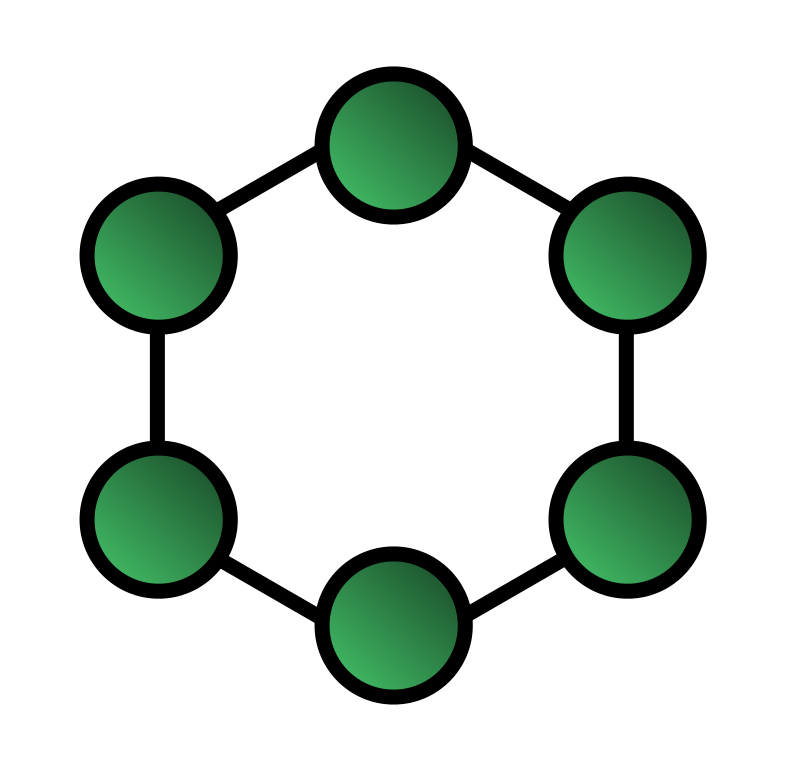
\includegraphics[width=7cm]{./RingNetwork.svg.PNG} \newline
\footnotetext{ Inc, S., (2002) . Networking Complete. Third Edition. San Francisco: Sybex }

\subsubsection{PROs}

\begin{itemize}
\item {When the load on the network increases, its performance is better than bus topology}
\item {There is no need of network server to control the connectivity between workstations}
\end{itemize}

\subsubsection{CONs}

\begin{itemize}
\item {Aggregate network bandwidth is bottlenecked by the weakest link between two nodes}
\end{itemize}

\clearpage
\printindex

\end{document}
